\begingroup
\raggedbottom
\chapter{离散时间傅里叶变换}
\label{chap:dtft}

离散时间信号 $x[n]$ 的时域自变量是整数，频域自变量仍可连续变化。\keyterm{离散时间傅里叶变换（discrete-time Fourier transform, DTFT）}用连续的频率描述序列中各复指数分量。本章采用 $X(\e^{\iu\omega})$ 记号；有限点\keyterm{离散傅里叶变换（DFT）}是另一种变换，不能由名称中的“离散”将两者混同。

\section{定义、周期性与收敛}
\label{sec:dtft-definition}

\subsection{正变换与逆变换}

\begin{definition}[离散时间傅里叶变换]
  对序列 $x[n]$，定义
  \begin{equation}
    X(\e^{\iu\omega})=\sum_{n=-\infty}^{\infty}x[n]\e^{-\iu\omega n}.
    \label{eq:dtft-definition}
  \end{equation}
  相应的逆变换为
  \begin{equation}
    x[n]=\frac{1}{2\pi}\int_{-\pi}^{\pi}
      X(\e^{\iu\omega})\e^{\iu\omega n}\dd\omega.
    \label{eq:dtft-inverse}
  \end{equation}
  记作 $x[n]\fourierpair X(\e^{\iu\omega})$。其中 $\omega$ 是离散时间角频率，单位为 $\mathrm{rad/sample}$，即每个样值间隔的弧度数。上述和式与积分\blue{须在相应的收敛意义下解释}。
\end{definition}

正变换对整数 $n$ 求和；逆变换\red{对连续频率积分}。频谱的记号 $\e^{\iu\omega}$ 表明它按单位圆上的位置取值；沿单位圆转过一周后频谱重复，\red{频率自变量仍连续}。幅度谱和相位谱的定义沿用\cref{sec:ctft-magnitude-phase}，只需把 $X(\iu\omega)$ 换成 $X(\e^{\iu\omega})$。

在 $\sum_n|x[n]|<\infty$ 时，将正变换代入逆变换，可交换求和与积分：
\begin{align*}
  \frac{1}{2\pi}\int_{-\pi}^{\pi}
    \left[\sum_{k=-\infty}^{\infty}x[k]\e^{-\iu\omega k}\right]
    \e^{\iu\omega n}\dd\omega
  &=\sum_{k=-\infty}^{\infty}x[k]\,
    \frac{1}{2\pi}\int_{-\pi}^{\pi}\e^{\iu\omega(n-k)}\dd\omega\\
  &=x[n].
\end{align*}
这里用到整数复指数的正交关系
\begin{equation}
  \frac{1}{2\pi}\int_{-\pi}^{\pi}\e^{\iu\omega(n-k)}\dd\omega
  =\begin{cases}1,&n=k,\\0,&n\ne k.\end{cases}
  \label{eq:dtft-orthogonality}
\end{equation}
$n=k$ 时被积函数为 $1$；$n\ne k$ 时，积分两端的指数相同，差为零。因此逆变换能\red{逐个恢复样值}，包括 $n=0$。

\subsection{频谱的周期与基本区间}
\label{sec:dtft-periodicity}

对任意整数 $r$，
\[
  \e^{\iu(\omega+2r\pi)n}=\e^{\iu\omega n},\qquad n\in\Z.
\]
由定义，
\begin{equation}
  X(\e^{\iu(\omega+2r\pi)})
  =\sum_n x[n]\e^{-\iu\omega n}\e^{-\iu2r\pi n}
  =X(\e^{\iu\omega}).
  \label{eq:dtft-periodicity}
\end{equation}
所以 DTFT 的频谱\red{必以二倍圆周率为周期}。$2\pi$ 未必是最小正周期，例如 $x[n]=\impulse[n]$ 的频谱恒为 $1$。

逆变换的被积函数 $X(\e^{\iu\omega})\e^{\iu\omega n}$ 同样以 $2\pi$ 为周期，积分区间可以改成任意一个长度为 $2\pi$ 的区间：
\[
  x[n]=\frac{1}{2\pi}\int_{\alpha}^{\alpha+2\pi}
    X(\e^{\iu\omega})\e^{\iu\omega n}\dd\omega.
\]
计算时\red{只积分一个完整周期}。对普通函数，有限个端点的取值不影响积分；若边界上有冲激，应把相邻周期的边界当作同一个频率点，\blue{不能重复计入}。选一个边界不经过谱线的区间通常更方便。

频率 $\omega$ 与 $\omega+2r\pi$ 对应同一个复指数序列。零频附近以及偶数倍 $\pi$ 附近都表示缓慢变化的分量，奇数倍 $\pi$ 附近则表示逐点快速交替的分量。\red{高低频按主周期判断}，不能仅凭 $|\omega|$ 的数值大小排序。特别地，
\[
  \e^{\iu\pi n}=\e^{-\iu\pi n}=(-1)^n,
\]
故 $\pi$ 与 $-\pi$ 是同一个离散时间频率。

\subsection{三种收敛意义}

\blue{绝对可和是充分条件}：
\[
  \sum_{n=-\infty}^{\infty}|x[n]|<\infty
  \quad\Longrightarrow\quad
  \sum_n\bigl|x[n]\e^{-\iu\omega n}\bigr|<\infty.
\]
此时变换对所有实数 $\omega$ 都收敛，而且频谱是\red{连续的周期函数}。有限长序列与满足 $|a|<1$ 的右侧指数序列都属于这一类。

若只满足 $\sum_n|x[n]|^2<\infty$，则可在\blue{均方意义下定义频谱}。例如后面的 sinc 型序列通常不绝对可和，却有有限能量，仍能得到周期矩形频谱；频谱跳跃处用对称极限取左右值的平均数。

常数、单位阶跃以及非零的正弦、余弦序列都没有有限能量，其 DTFT \red{要在广义函数意义下解释}。\blue{不收敛时先辨认意义}，不能把发散级数直接套进无限等比级数公式。含冲激的频谱仍用\cref{eq:dtft-inverse} 反演，相关判等约定见\cref{chap:math-foundations}。

\section{典型序列的傅里叶变换}
\label{sec:dtft-basic-pairs}

以下变换对依次为右侧指数、单位冲激、常数、有限长矩形、sinc 型序列、单位阶跃、正余弦和符号序列。冲激 $\impulse[n]$ 是离散时间单位样值；频域的 $\impulse(\omega-\omega_0)$ 则是连续频率变量上的狄拉克冲激，箭头旁标的是权重。

\subsection{右侧衰减指数序列}
\label{sec:dtft-exponential}

对 $|a|<1$，
\begin{equation}
  \boxed{a^n\stepfun[n]\fourierpair\frac{1}{1-a\e^{-\iu\omega}}}.
  \label{eq:dtft-exponential}
\end{equation}
这里序列在 $n<0$ 时为零，在 $n\ge0$ 时为 $a^n$。若 $a=0$，约定 $x[0]=1$、其余样值为零。直接求和：
\[
  X(\e^{\iu\omega})
  =\sum_{n=0}^{\infty}(a\e^{-\iu\omega})^n
  =\lim_{N\to\infty}\frac{1-(a\e^{-\iu\omega})^{N+1}}
    {1-a\e^{-\iu\omega}}
  =\frac{1}{1-a\e^{-\iu\omega}}.
\]
等比级数收敛要求\red{公比的模小于一}，与 $\omega$ 无关。

对实数 $-1<a<1$，
\begin{align*}
  X(\e^{\iu\omega})
    &=\frac{1}{1-a\cos\omega+\iu a\sin\omega},\\
  |X(\e^{\iu\omega})|^2
    &=\frac{1}{1+a^2-2a\cos\omega},\\
  |X(\e^{\iu\omega})|
    &=\frac{1}{\sqrt{1+a^2-2a\cos\omega}},\\
  \theta(\omega)
    &=-\arctan\frac{a\sin\omega}{1-a\cos\omega}.
\end{align*}
因为 $1-a\cos\omega>0$，最后一式可以直接采用通常的反正切主值。负号来自取倒数；幅度和相位都随频率周期重复。

$0<a<1$ 时，幅度在 $\omega=2r\pi$ 处最大，峰值为 $1/(1-a)$。$-1<a<0$ 时，样值正负交替，幅度峰值移到奇数倍 $\pi$，为 $1/(1-|a|)$。\red{负参数对应交替样值}，两种参数的幅相谱见\cref{fig:dtft-exponential}。
\begin{figure}[H]
  \centering
  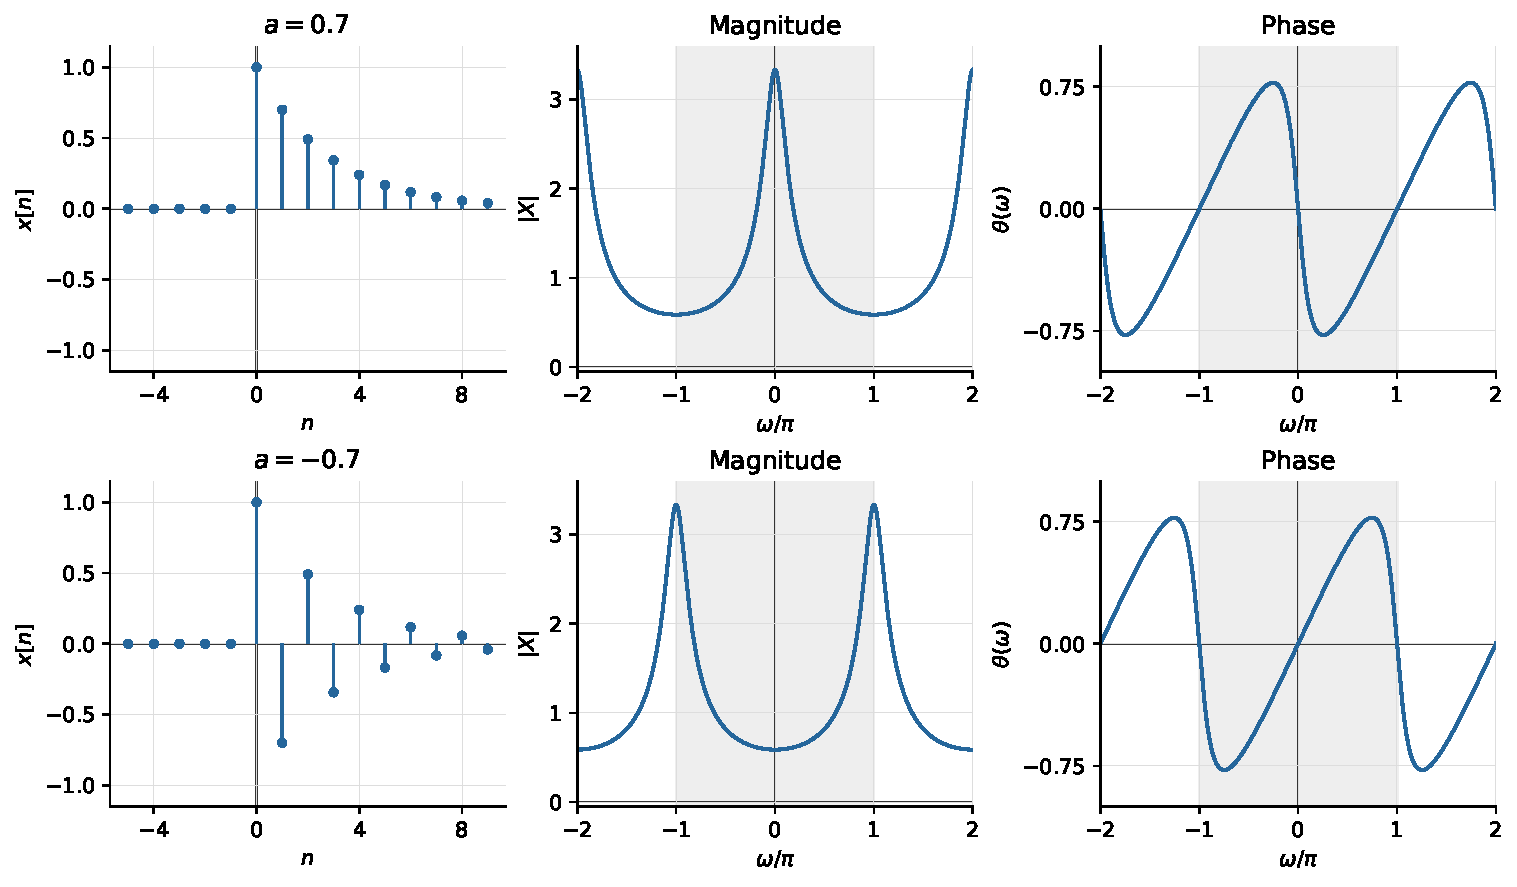
\includegraphics[width=0.98\textwidth]{07-dtft/exponential.pdf}
  \caption{右侧指数序列及其幅度谱、相位谱，上行 $a=0.7$，下行 $a=-0.7$。频率横轴以 $\pi$ 归一化，灰色区域标出一个基本周期。}
  \label{fig:dtft-exponential}
\end{figure}

\subsection{单位冲激序列}

\begin{equation}
  \boxed{\impulse[n]\fourierpair1}.
  \label{eq:dtft-impulse}
\end{equation}
由定义，
\[
  X(\e^{\iu\omega})=\sum_n\impulse[n]\e^{-\iu\omega n}=1.
\]
它的\red{幅度谱处处为一}，相位处处为零。逆向核对时，\cref{eq:dtft-orthogonality} 给出
$\frac1{2\pi}\int_{-\pi}^{\pi}\e^{\iu\omega n}\dd\omega=\impulse[n]$。
时域只改变零点样值，频域就叠加一个\red{覆盖全部频率的常数}，见\cref{fig:dtft-impulse-constant} 上行。因此\blue{零点样值不能忽略}。

\subsection{常数序列}

\begin{equation}
  \boxed{1\fourierpair
    2\pi\sum_{r=-\infty}^{\infty}\impulse(\omega-2r\pi)}.
  \label{eq:dtft-constant}
\end{equation}
在 $(-\pi,\pi)$ 内只有 $\omega=0$ 这一条谱线，故
\[
  x[n]=\frac1{2\pi}\int_{-\pi}^{\pi}
    2\pi\impulse(\omega)\e^{\iu\omega n}\dd\omega=1.
\]
频谱的\red{每周期有一条直流谱线}，每条权重为 $2\pi$。画一个主周期时可只画零频冲激，但完整频谱必须\red{延拓为周期冲激串}，不能写成全频轴上仅有 $2\pi\impulse(\omega)$，见\cref{fig:dtft-impulse-constant} 下行。
\begin{figure}[H]
  \centering
  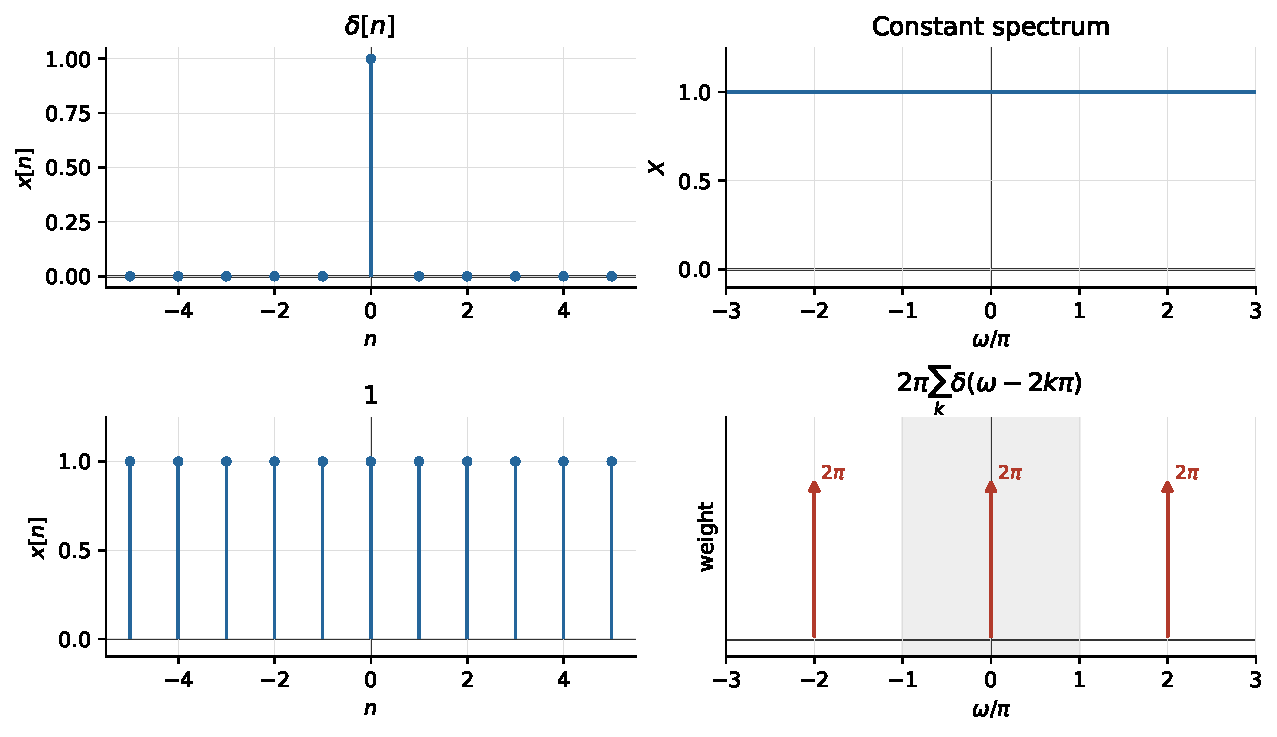
\includegraphics[width=0.92\textwidth]{07-dtft/impulse-constant.pdf}
  \caption{离散单位冲激与常数序列。时域竖线表示样值；频域箭头表示连续频率上的冲激，其权重为 $2\pi$。}
  \label{fig:dtft-impulse-constant}
\end{figure}

\subsection{有限长对称矩形序列}
\label{sec:dtft-rectangle}

设 $N_1$ 为非负整数，
\[
  x[n]=\begin{cases}1,&-N_1\le n\le N_1,\\0,&\text{其他}.\end{cases}
\]
序列共有 $2N_1+1$ 个非零样值。利用有限等比级数，
\begin{align*}
  X(\e^{\iu\omega})
  &=\sum_{n=-N_1}^{N_1}\e^{-\iu\omega n}
    =1+2\sum_{n=1}^{N_1}\cos(n\omega)\\
  &=\e^{\iu N_1\omega}\frac{1-\e^{-\iu(2N_1+1)\omega}}
    {1-\e^{-\iu\omega}}
    =\frac{\sin\bigl((N_1+\tfrac12)\omega\bigr)}
      {\sin(\omega/2)}.
\end{align*}
于是
\begin{equation}
  \boxed{\mathbf 1_{|n|\le N_1}\fourierpair
    \frac{\sin\bigl((N_1+\tfrac12)\omega\bigr)}{\sin(\omega/2)}}.
  \label{eq:dtft-rectangle}
\end{equation}
$\omega=2r\pi$ 处是\blue{可去奇点须补值}：
\[
  X(\e^{\iu2r\pi})=2N_1+1.
\]
这个值也可直接由有限和式得到，等于全部样值之和。$N_1\ge1$ 时，其他零点为
$\omega=2k\pi/(2N_1+1)$，其中 $k$ 不为 $2N_1+1$ 的整数倍。零频主瓣宽度为 $4\pi/(2N_1+1)$，所以\red{序列越长，主瓣越窄}。

频谱为带符号的实函数，\red{幅度谱须取绝对值}；正瓣的相位为 $0$，负瓣可取 $\pi$，零点处没有相位。\cref{fig:dtft-rectangle} 取 $N_1=2$，此时 $X=1+2\cos\omega+2\cos2\omega$。与连续矩形的 sinc 频谱相比，这里的分母为 $\sin(\omega/2)$，频谱周期重复。
\begin{figure}[H]
  \centering
  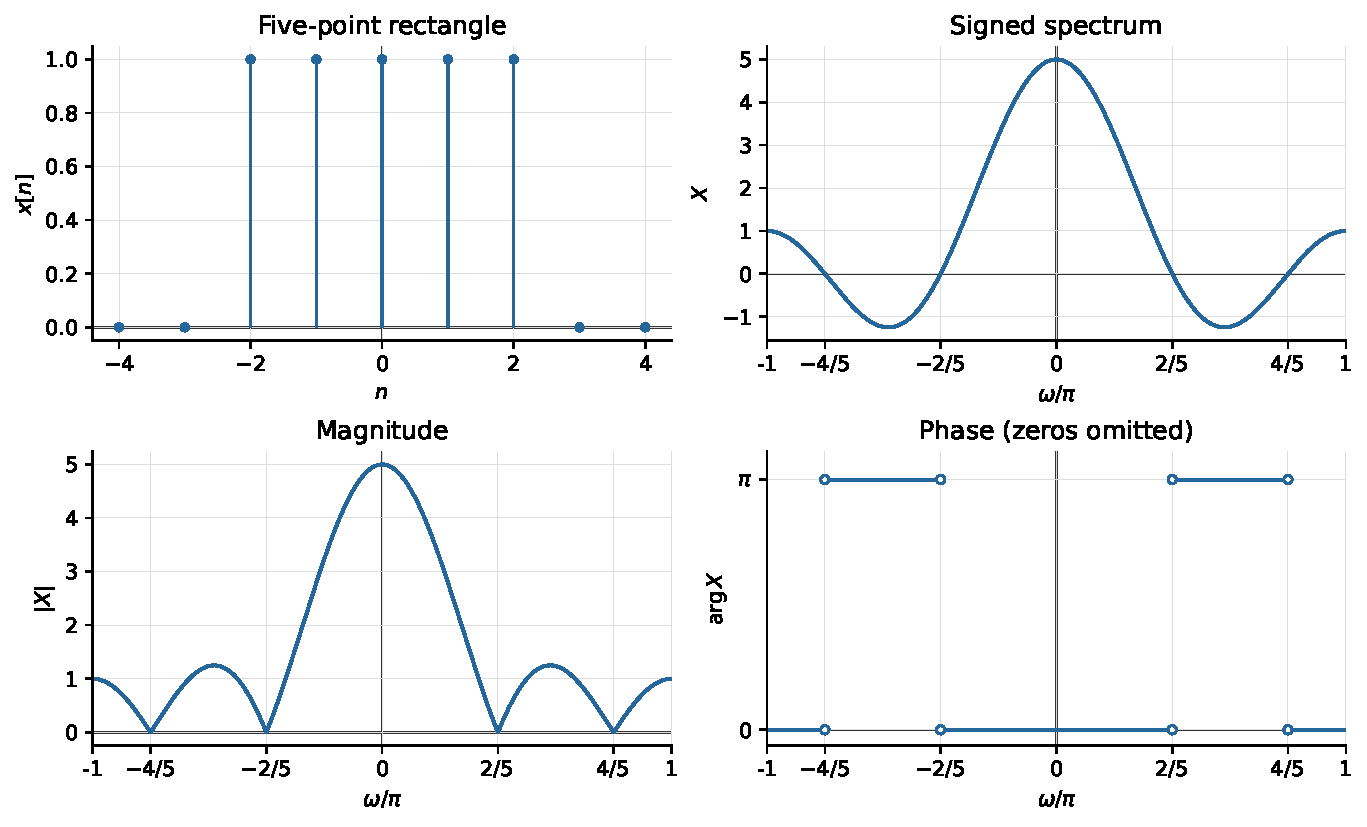
\includegraphics[width=0.96\textwidth]{07-dtft/rectangle.pdf}
  \caption{五点矩形序列及其带符号频谱、幅度谱和相位谱。相位图在频谱零点处留空。}
  \label{fig:dtft-rectangle}
\end{figure}

\subsection{sinc 型序列与周期矩形频谱}
\label{sec:dtft-sinc}

对 $0<\omega_0<\pi$，定义
\begin{equation}
  s_{\omega_0}[n]=
  \begin{cases}
    \dfrac{\sin(\omega_0 n)}{\pi n},&n\ne0,\\[3pt]
    \dfrac{\omega_0}{\pi},&n=0.
  \end{cases}
  \label{eq:dtft-sinc-sequence}
\end{equation}
它的变换为
\begin{equation}
  \boxed{s_{\omega_0}[n]\fourierpair R_{\omega_0}(\omega)},\qquad
  R_{\omega_0}(\omega)=
  \begin{cases}
    1,&|\omega|<\omega_0,\\
    0,&\omega_0<|\omega|<\pi,
  \end{cases}
  \label{eq:dtft-sinc-pair}
\end{equation}
并规定 $R_{\omega_0}(\omega+2\pi)=R_{\omega_0}(\omega)$。
从矩形频谱作逆变换，$n\ne0$ 时
\[
  x[n]=\frac{1}{2\pi}\int_{-\omega_0}^{\omega_0}
    \e^{\iu\omega n}\dd\omega
  =\frac{\sin(\omega_0 n)}{\pi n}.
\]
$n=0$ 时直接积分得到 $\omega_0/\pi$，与把 $n$ 暂看成连续变量求极限的结果一致。\red{中心值由频谱面积确定}，不能因表达式出现 $0/0$ 就将它置零。频域边界 $\omega=\pm\omega_0+2r\pi$ 采用对称求和时取 $1/2$；有限个\blue{边界点的取值不影响反演}。

\cref{fig:dtft-sinc} 对比 $\omega_0=\pi/4$ 与 $3\pi/4$。序列是连续 sinc 曲线在整数点的样值，频谱则是\red{周期延拓的矩形}。参数为 $3\pi/4$ 时，矩形半宽为 $3\pi/4$，$s[0]=3/4$；取 $-\pi/4$ 时序列整体反号，矩形高度也变成 $-1$。
\begin{figure}[H]
  \centering
  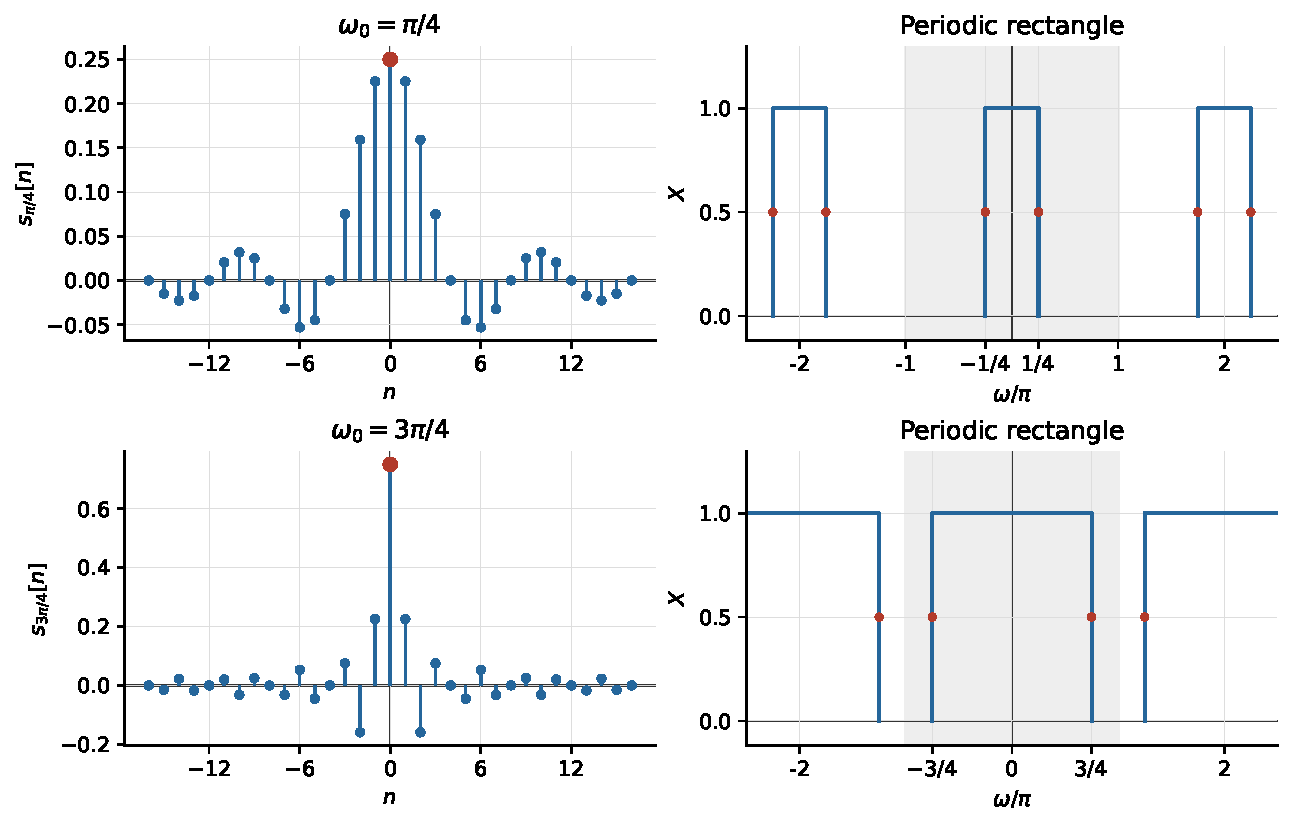
\includegraphics[width=0.92\textwidth]{07-dtft/sinc.pdf}
  \caption{$s_{\pi/4}[n]$ 与 $s_{3\pi/4}[n]$ 及其周期矩形频谱。零点样值分别为 $1/4$、$3/4$；频谱跳跃处按对称极限取 $1/2$。}
  \label{fig:dtft-sinc}
\end{figure}

连续 sinc 的矩形频谱可以在频率轴上任意展宽；此处公式的直接使用范围是 $0<\omega_0<\pi$。超出这一范围后的零点修正与矩形重叠见\cref{sec:dtft-sinc-tips}。

\subsection{单位阶跃序列}
\label{sec:dtft-step}

离散单位阶跃满足 $\stepfun[0]=1$，其 DTFT 为
\begin{equation}
  \boxed{\stepfun[n]\fourierpair
    \operatorname{pv}\frac{1}{1-\e^{-\iu\omega}}
    +\pi\sum_{k=-\infty}^{\infty}\impulse(\omega-2k\pi)}.
  \label{eq:dtft-step}
\end{equation}
其中 $\operatorname{pv}$ 表示在每个周期奇点附近取\keyterm{对称主值}。在 $\omega\ne2k\pi$ 处，
\[
  \frac{1}{1-\e^{-\iu\omega}}
  =\frac12-\frac{\iu}{2}\cot\frac{\omega}{2}.
\]
实部含常数 $1/2$ 和权重 $\pi$ 的周期冲激，虚部为 $-\frac12\operatorname{pv}\cot(\omega/2)$。\red{阶跃频谱须保留冲激}，\blue{不能只写这个分式}。

为推导该式，先取 $0<r<1$ 的衰减序列 $r^n\stepfun[n]$。其频谱的实部、虚部为
\[
  \Re X_r=\frac12+\frac{1-r^2}{2(1-2r\cos\omega+r^2)},
  \qquad
  \Im X_r=-\frac{r\sin\omega}{1-2r\cos\omega+r^2}.
\]
实部的第二项在一个周期上的积分为 $\pi$；当 $r\to1^-$ 时，它集中到 $\omega=0$ 及其周期副本，趋于 $\pi\sum_k\impulse(\omega-2k\pi)$。虚部趋于主值余切。这里\red{极限按广义函数理解}；逐点求极限会漏掉集中的冲激质量。

若改用有限长截断 $u_N[n]=1$（$0\le n\le N$），则
\[
  U_N(\e^{\iu\omega})
  =\sum_{n=0}^{N}\e^{-\iu\omega n}
  =\frac{1-\e^{-\iu\omega(N+1)}}{1-\e^{-\iu\omega}}.
\]
在 $\omega=2k\pi$ 处按有限和补值 $N+1$。$N\to\infty$ 时，分子中的指数项通常没有逐点极限；整个 $U_N$ 在分布意义下才趋于\cref{eq:dtft-step}。衰减法和截断法得到同一个阶跃频谱。

在 $n=0$ 处逆变换，常数实部贡献 $1/2$，周期冲激贡献 $1/2$，奇的虚部积分为零，所以恢复出 $\stepfun[0]=1$。这与连续阶跃在跳跃处取左右平均值的情形不同：离散时间的\red{单个样值必须恢复}。频谱各部分见\cref{fig:dtft-step}。
\begin{figure}[H]
  \centering
  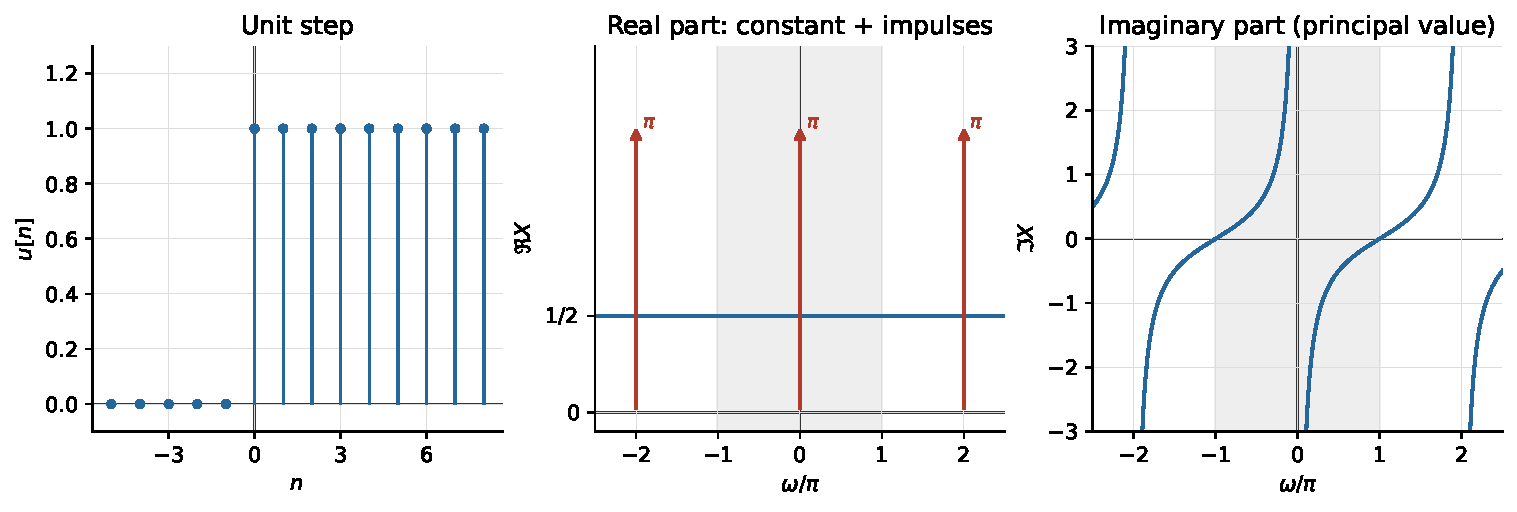
\includegraphics[width=0.98\textwidth]{07-dtft/step.pdf}
  \caption{单位阶跃序列及其频谱实部、虚部。实部的水平线为 $1/2$，箭头权重为 $\pi$；虚部在各奇点断开，按周期主值理解。}
  \label{fig:dtft-step}
\end{figure}

\subsection{复指数、余弦与正弦序列}
\label{sec:dtft-harmonics}

单一复指数的变换为
\begin{equation}
  \boxed{\e^{\iu\omega_0 n}\fourierpair
    2\pi\sum_{r=-\infty}^{\infty}
      \impulse(\omega-\omega_0-2r\pi)}.
  \label{eq:dtft-complex-exponential}
\end{equation}
选一个只含 $\omega_0$ 的长度为 $2\pi$ 的区间反演，
$x[n]=(2\pi)^{-1}2\pi\e^{\iu\omega_0n}$，即可核对权重。该公式对任意实数 $\omega_0$ 成立，即使 $\omega_0/(2\pi)$ 为无理数、\blue{时域序列不周期}，频谱仍以 $2\pi$ 为周期。

由欧拉公式，
\begin{align}
  \cos(\omega_0 n)&\fourierpair
    \pi\sum_{r=-\infty}^{\infty}
      \left[\impulse(\omega-\omega_0-2r\pi)
        +\impulse(\omega+\omega_0-2r\pi)\right],
    \label{eq:dtft-cosine}\\
  \sin(\omega_0 n)&\fourierpair
    \frac{\pi}{\iu}\sum_{r=-\infty}^{\infty}
      \left[\impulse(\omega-\omega_0-2r\pi)
        -\impulse(\omega+\omega_0-2r\pi)\right].
    \label{eq:dtft-sine}
\end{align}
$0<\omega_0<\pi$ 时，一个主周期内有两条不同的谱线。余弦的两条权重均为 $\pi$；正弦在 $+\omega_0$ 处为 $-\iu\pi$，在 $-\omega_0$ 处为 $+\iu\pi$。\red{正弦谱线权重为虚数}，画图须标清画的是虚部；对应谱线相位分别为 $-\pi/2$ 和 $\pi/2$，见\cref{fig:dtft-harmonics}。谱线幅度指权重的模，均为 $\pi$。

\begin{figure}[H]
  \centering
  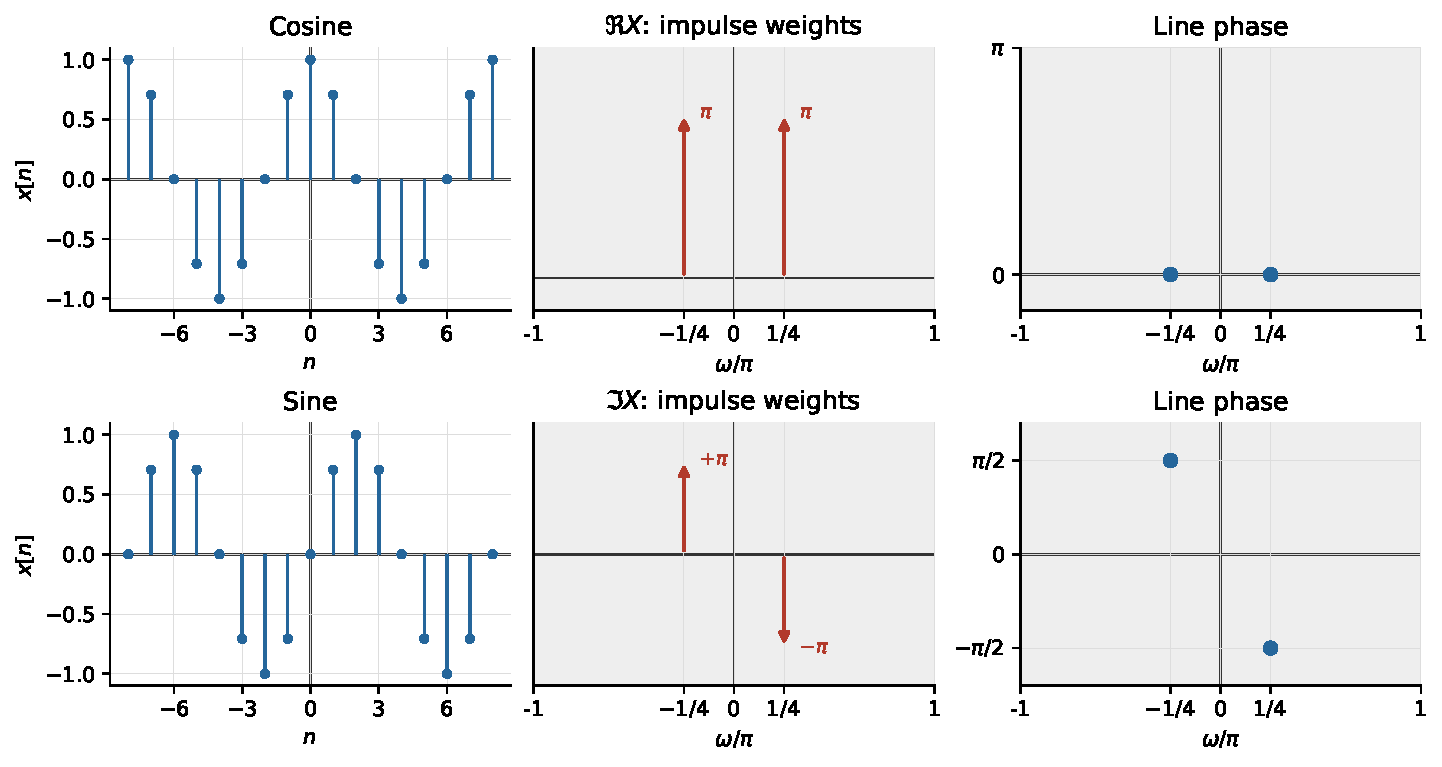
\includegraphics[width=0.98\textwidth]{07-dtft/harmonics.pdf}
  \caption{$\omega_0=\pi/4$ 的余弦与正弦序列。中列分别画频谱的实部和虚部，箭头旁标权重；右列只在谱线上标相位。}
  \label{fig:dtft-harmonics}
\end{figure}

例如 $\cos(9\pi n/4)=\cos(\pi n/4)$，\red{两者频谱完全相同}。参数为 $\pi$ 时，两个谱线族重合：
\begin{equation}
  \cos(\pi n)=\e^{\iu\pi n}=\e^{-\iu\pi n}=(-1)^n
  \fourierpair
  2\pi\sum_{r=-\infty}^{\infty}\impulse\bigl(\omega-(2r+1)\pi\bigr).
  \label{eq:dtft-alternating}
\end{equation}
余弦的两份权重在同一位置相加为 $2\pi$；正弦的两份权重相消，
$\sin(\pi n)=0$，其频谱也为零。\hl{重合谱线先合并权重}。在 $[-\pi,\pi]$ 上绘图时，两端属于同一个基本周期的边界点，\hl{边界谱线不能算两次}。为便于读取，\cref{fig:dtft-alternating} 显示了多个周期。
\begin{figure}[H]
  \centering
  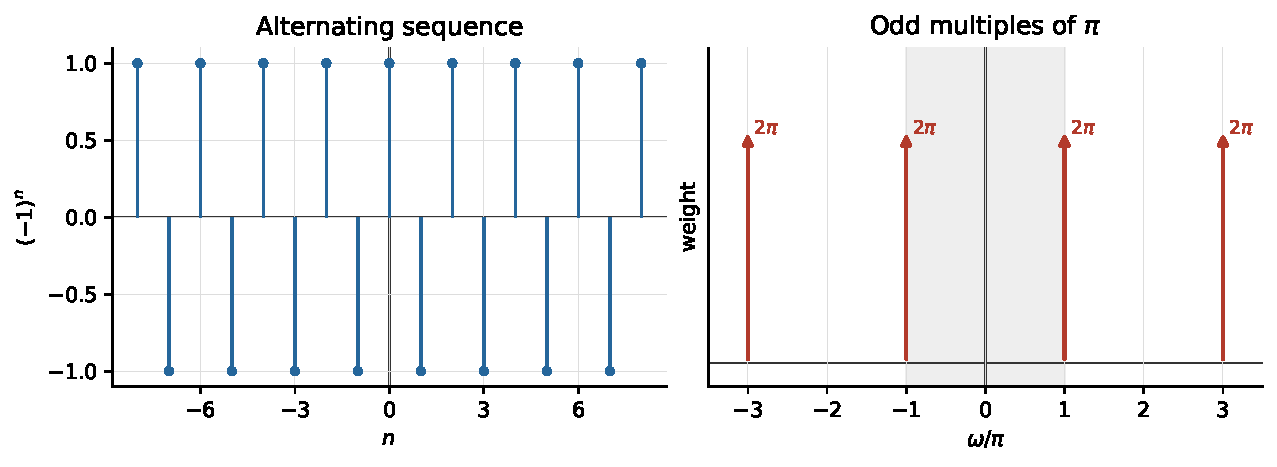
\includegraphics[width=0.92\textwidth]{07-dtft/alternating.pdf}
  \caption{$(-1)^n$ 及其周期冲激谱。奇数倍 $\pi$ 处的权重为 $2\pi$；一个基本周期只含一条等价谱线。}
  \label{fig:dtft-alternating}
\end{figure}

\subsection{符号序列}
\label{sec:dtft-sign}

离散符号序列定义为
\[
  \operatorname{sgn}(n)=
  \begin{cases}1,&n>0,\\0,&n=0,\\-1,&n<0.\end{cases}
\]
它与单位阶跃的关系是
\[
  \operatorname{sgn}(n)=2\stepfun[n]-1-\impulse[n].
\]
因为 $\stepfun[0]=1$，\red{零点须减去单位样值}，才能得到 $\operatorname{sgn}(0)=0$。将三项分别变换，周期冲激串相消：
\begin{align*}
  S(\e^{\iu\omega})
    &=2\left(\operatorname{pv}\frac1{1-\e^{-\iu\omega}}
        +\pi\sum_k\impulse(\omega-2k\pi)\right)
      -2\pi\sum_k\impulse(\omega-2k\pi)-1\\
    &=\operatorname{pv}\frac{1+\e^{-\iu\omega}}{1-\e^{-\iu\omega}}.
\end{align*}
用分子、分母共同的因子 $\e^{-\iu\omega/2}$ 化简，得到
\begin{equation}
  \boxed{\operatorname{sgn}(n)\fourierpair
    -\iu\operatorname{pv}\cot\frac{\omega}{2}}.
  \label{eq:dtft-sign}
\end{equation}
也可写成 $-\iu/\tan(\omega/2)$，\blue{奇点仍按周期主值理解}。序列是实奇序列，频谱为\red{纯虚的奇函数}。在普通函数部分，幅度为 $|\cot(\omega/2)|$；在主周期内，$-\pi<\omega<0$ 时相位为 $\pi/2$，$0<\omega<\pi$ 时为 $-\pi/2$。奇数倍 $\pi$ 处频谱为零，相位未定义；偶数倍 $\pi$ 处是主值奇点，不能赋予有限的幅度或相位。对应图像见\cref{fig:dtft-sign}。
\begin{figure}[H]
  \centering
  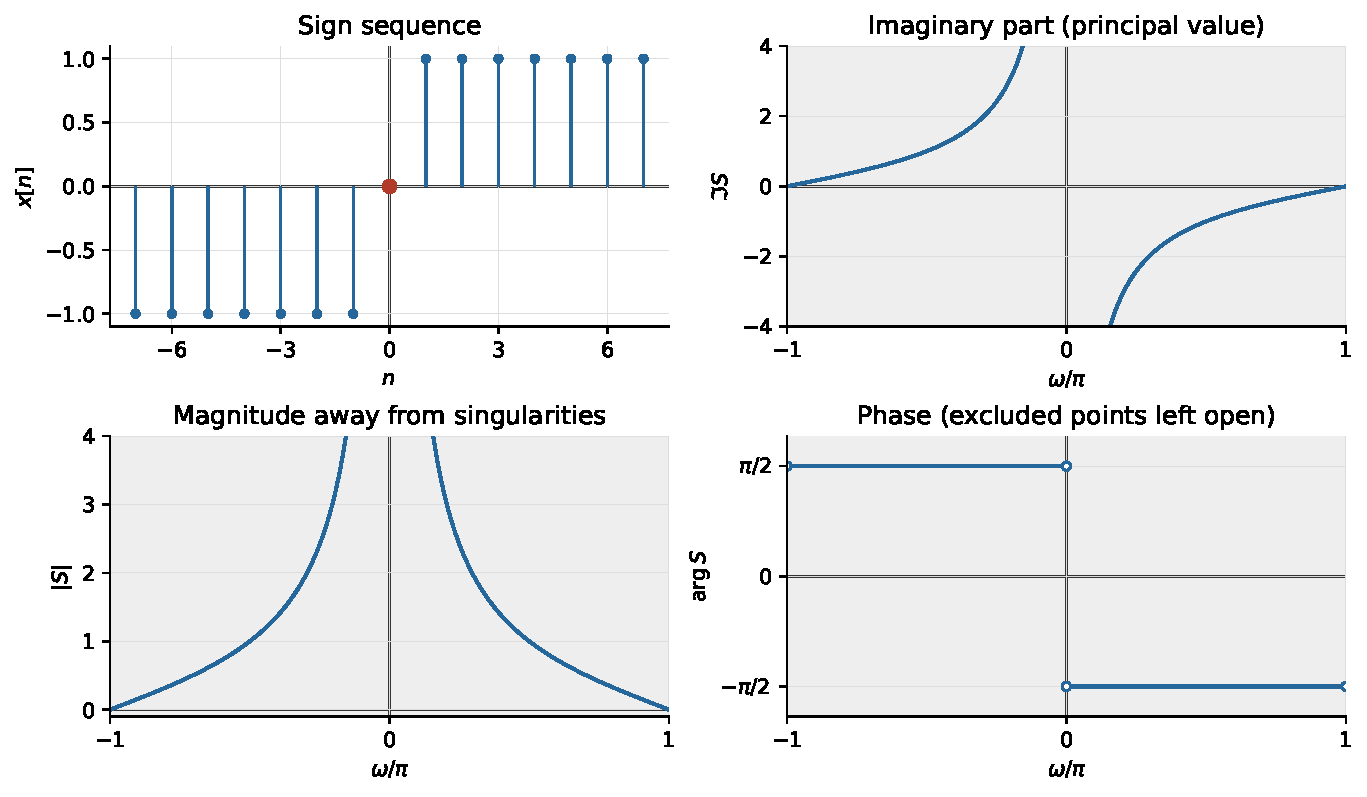
\includegraphics[width=0.96\textwidth]{07-dtft/sign.pdf}
  \caption{符号序列及其频谱虚部、普通函数部分的幅度与相位。奇点处曲线断开，零频两侧按周期主值理解；相位图省略奇点与零点。}
  \label{fig:dtft-sign}
\end{figure}

\section{变换对中的参数与易错点}
\label{sec:dtft-pair-tips}

\subsection{sinc 参数超出主周期时}
\label{sec:dtft-sinc-tips}

将\cref{eq:dtft-sinc-sequence} 中的参数推广为任意实数 $\gamma$，仍规定
$s_\gamma[0]=\gamma/\pi$。对 $n\ne0$，整数性给出
$\sin((\gamma+2q\pi)n)=\sin(\gamma n)$；零点样值却增加 $2q$。因此
\begin{equation}
  s_{\gamma+2q\pi}[n]=s_\gamma[n]+2q\impulse[n],
  \qquad q\in\Z.
  \label{eq:dtft-sinc-parameter-wrap}
\end{equation}
\red{非零样值相同仍须查零点}。零点修正 $2q\impulse[n]$ 的变换是常数 $2q$，\red{零点修正对应常数频谱}。

两个具体参数为
\begin{align}
  s_{5\pi/4}[n]&=-s_{3\pi/4}[n]+2\impulse[n]
    \fourierpair 2-R_{3\pi/4}(\omega),
    \label{eq:dtft-sinc-five-fourths}\\
  s_{9\pi/4}[n]&=s_{\pi/4}[n]+2\impulse[n]
    \fourierpair 2+R_{\pi/4}(\omega).
    \label{eq:dtft-sinc-nine-fourths}
\end{align}
在 $n=0$ 处，第一式为 $-3/4+2=5/4$，第二式为 $1/4+2=9/4$。第一式在主周期中央高度为 $1$、两侧为 $2$；第二式中央高度为 $3$、两侧为 $2$，均为普通函数频谱。负参数的反号及这两种重叠见\cref{fig:dtft-sinc-parameters}。

\begin{figure}[H]
  \centering
  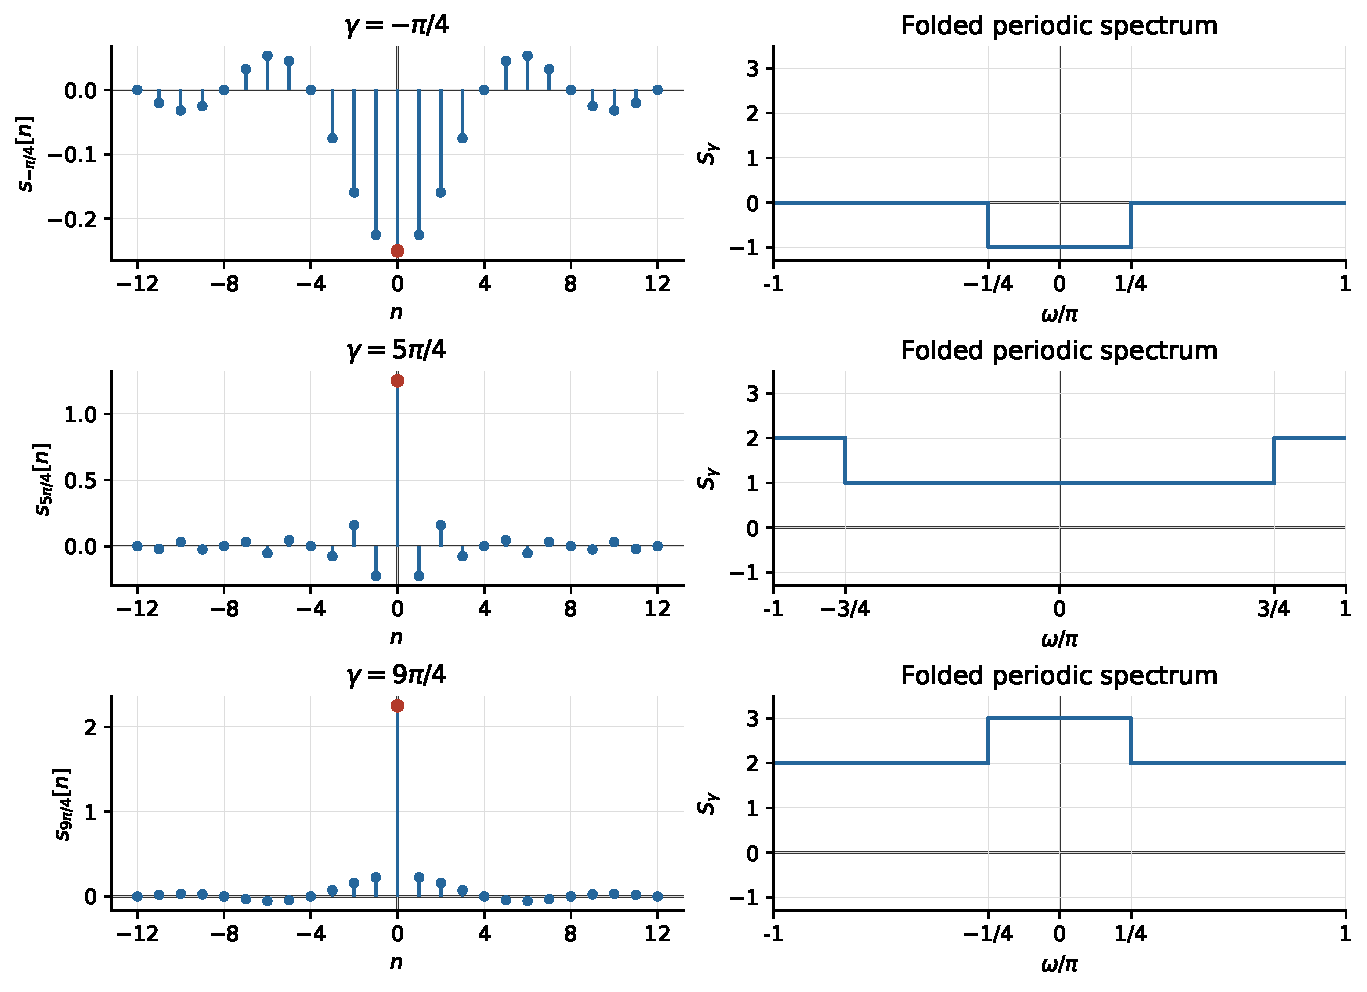
\includegraphics[width=0.96\textwidth]{07-dtft/sinc-parameters.pdf}
  \caption{参数 $-\pi/4$、$5\pi/4$、$9\pi/4$ 的 sinc 型序列及频谱。左列红点标出零点样值；右列为带符号的频谱值。}
  \label{fig:dtft-sinc-parameters}
\end{figure}

还可从逆变换直接理解重叠。对 $\gamma>0$，
\[
  s_\gamma[n]=\frac{1}{2\pi}\int_{-\gamma}^{\gamma}
    \e^{\iu\omega n}\dd\omega.
\]
把长区间中的各段平移整数倍 $2\pi$，折回一个基本周期后，被积指数不变，各段覆盖次数相加。所以频谱可表示成
\[
  S_\gamma(\omega)=\sum_{q=-\infty}^{\infty}
    \mathbf 1_{|\omega-2q\pi|<\gamma},
\]
边界按平均值处理。\red{重叠区域的高度相加}；$\gamma<\pi$ 时副本不重叠，才得到高度为 $1$ 的单个周期矩形。若 $\gamma<0$，再用 $s_\gamma=-s_{-\gamma}$。

\subsection{sinc 求和与连续积分}

取 DTFT 的零频值得到
\begin{equation}
  \lim_{N\to\infty}\sum_{n=-N}^{N}
    \frac{\sin(\gamma n)}{\pi n}
  =\begin{cases}
    1,&0<\gamma<\pi,\\
    0,&\gamma=0,\\
    -1,&-\pi<\gamma<0.
  \end{cases}
  \label{eq:dtft-sinc-sum}
\end{equation}
式中 $n=0$ 的项必须按 $\gamma/\pi$ 补上，\blue{求和按对称极限理解}。该式的\red{参数范围不能删去}；超出主周期时应使用前一小节的重叠频谱。例如 $\gamma=9\pi/4$ 时，零频值为 $3$。

若只对非零整数求和，\blue{就须减去零点项}：
\begin{equation}
  \lim_{N\to\infty}\sum_{\substack{n=-N\\n\ne0}}^{N}
    \frac{\sin(\gamma n)}{\pi n}
  =\operatorname{sgn}(\gamma)-\frac{\gamma}{\pi},
  \qquad 0<|\gamma|<\pi.
  \label{eq:dtft-sinc-sum-without-zero}
\end{equation}
\red{省略零点会改变结果}。在 $\gamma=\pi$ 时，非零样值全部为零，零点样值为 $1$，故 $s_\pi[n]=\impulse[n]$；参数为 $-\pi$ 时为 $-\impulse[n]$。

连续时间对应的振荡积分为
\[
  \int_{-\infty}^{\infty}\frac{\sin(\gamma t)}{\pi t}\dd t
  =\operatorname{sgn}(\gamma),\qquad \operatorname{sgn}(0)=0,
\]
见\cref{sec:ctft-sinc-pair}。连续积分对任意实数 $\gamma$ 都有这一形式；离散求和受周期频谱的重叠影响。连续积分中单点的取值不改变面积，离散求和中 $n=0$ 的项则必须计入。

\subsection{指数、阶跃与两种频率变量}

连续与离散右侧指数的变换分别见\cref{eq:ctft-exponential-pair,eq:dtft-exponential}：
\[
  \e^{-\alpha t}\stepfun(t)\fourierpair\frac1{\alpha+\iu\Omega},
  \quad\alpha>0;
  \qquad
  a^n\stepfun[n]\fourierpair\frac1{1-a\e^{-\iu\omega}},
  \quad |a|<1.
\]
这里用 $\Omega$ 区分连续时间角频率，单位为 $\mathrm{rad/s}$。采样间隔为 $T$ 时，复指数在 $t=nT$ 处取值为 $\e^{\iu\Omega Tn}$，所以 $\omega=\Omega T$，并按 $2\pi$ 等价。\red{两种频率单位不同}。

指数趋向阶跃时，连续情形取 $\alpha\to0^+$，离散情形取 $a\to1^-$。两者都超出了普通积分或绝对可和级数的收敛范围，\red{边界极限会出现冲激}。连续阶跃带单个 $\pi\impulse(\Omega)$，离散阶跃带周期冲激串，见\cref{eq:ctft-step-pair,eq:dtft-step}。直接代入 $\alpha=0$ 或 $a=1$，会漏掉这一项。

正弦、余弦与 sinc 型序列都可能含有参数 $\omega_0$，但化简规则要检查整个表达式。正余弦的频率加 $2\pi$ 后全序列相同；sinc 型序列的非零样值相同，零点样值可能不同。作参数化简前，\blue{检查定义中的零点约定}。

\section{傅里叶变换的基本性质}
\label{sec:dtft-properties}

本节沿用\cref{eq:dtft-definition,eq:dtft-inverse} 的变换约定。时移和频移可直接由定义推得；差分、卷积与累加则把时域运算转成频域中的乘法。涉及无穷和的换序或逐项求导时，须检查收敛条件。

\subsection{线性性质}

若 $x_1[n]\fourierpair X_1(\e^{\iu\omega})$、$x_2[n]\fourierpair X_2(\e^{\iu\omega})$，则对常数 $a,b$，
\begin{equation}
  a x_1[n]+b x_2[n]\fourierpair
  aX_1(\e^{\iu\omega})+bX_2(\e^{\iu\omega}).
  \label{eq:dtft-linearity}
\end{equation}
将线性组合代入定义，拆开求和便得到该式。\red{相加的是复频谱}，不能直接把幅度谱相加；相位不同的分量可能抵消。

\begin{example}[sinc 序列与冲激的叠加]
  用\cref{eq:dtft-sinc-pair,eq:dtft-impulse}，
  \[
    s_{\pi/4}[n]+\impulse[n]\fourierpair R_{\pi/4}(\omega)+1.
  \]
  一个主周期内，中央 $|\omega|<\pi/4$ 的高度为 $2$，其余部分为 $1$，见\cref{fig:dtft-linear-sum}。时域只把 $n=0$ 的样值由 $1/4$ 改为 $5/4$，频域则\red{整个背景增加一}。
  \begin{figure}[H]
    \centering
    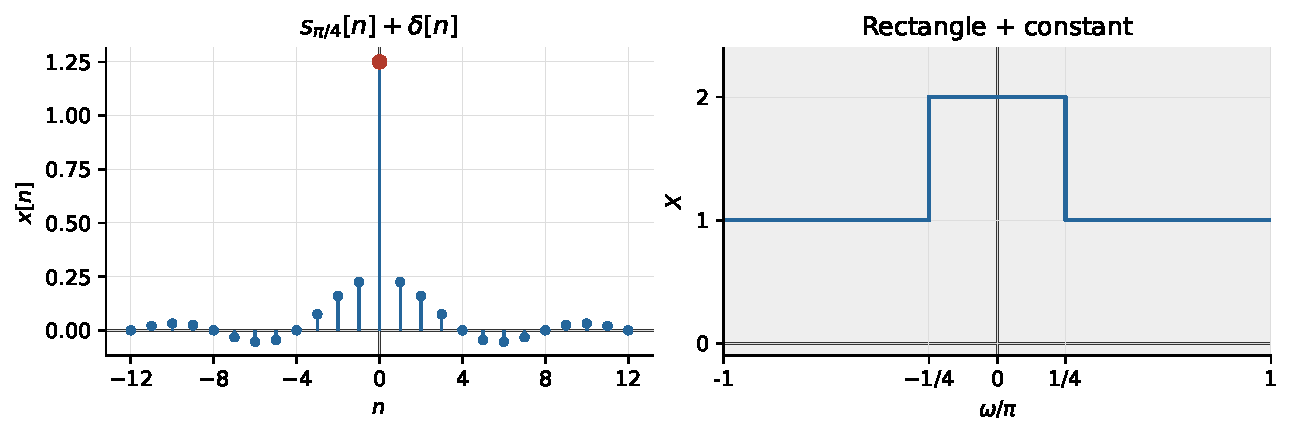
\includegraphics[width=0.86\textwidth]{07-dtft/linear-sum.pdf}
    \caption{sinc 序列叠加单位冲激后的样值与频谱。频域增加的是常数背景。}
    \label{fig:dtft-linear-sum}
  \end{figure}
\end{example}

\subsection{时移与频移}
\label{sec:dtft-shifts}

对整数 $n_0$，
\begin{equation}
  x[n-n_0]\fourierpair
  \e^{-\iu\omega n_0}X(\e^{\iu\omega}).
  \label{eq:dtft-time-shift}
\end{equation}
令 $m=n-n_0$，则
\[
  \sum_n x[n-n_0]\e^{-\iu\omega n}
  =\sum_m x[m]\e^{-\iu\omega(m+n_0)}
  =\e^{-\iu\omega n_0}X(\e^{\iu\omega}).
\]
时移\red{保留幅度，改变相位}：相位增加 $-\omega n_0$，并按 $2\pi$ 等价。$n_0>0$ 表示延迟，增加的线性相位斜率为负；频谱为零处仍没有相位。整数条件同时保证乘子 $\e^{-\iu\omega n_0}$ 以 $2\pi$ 为周期。连续时间的对应式见\cref{eq:ctft-time-shift}，其中时移量可为任意实数。

对任意实数 $\omega_0$，
\begin{equation}
  \e^{\iu\omega_0 n}x[n]\fourierpair
  X\bigl(\e^{\iu(\omega-\omega_0)}\bigr).
  \label{eq:dtft-frequency-shift}
\end{equation}
直接合并指数：
\[
  \sum_n \e^{\iu\omega_0n}x[n]\e^{-\iu\omega n}
  =\sum_n x[n]\e^{-\iu(\omega-\omega_0)n}
  =X\bigl(\e^{\iu(\omega-\omega_0)}\bigr).
\]
乘以正频率复指数，把频谱向右移 $\omega_0$。画主周期时，\red{越过边界须周期折回}，\blue{不能截掉越界部分}。\cref{fig:dtft-shifts} 分别展示延迟的幅相变化与跨越 $\pi$ 边界的频移。低通矩形平移 $\pi$ 后成为高通的计算已在\cref{ex:dtft-highpass} 给出；此时乘子是 $\e^{\iu\pi n}=(-1)^n$。
\begin{figure}[H]
  \centering
  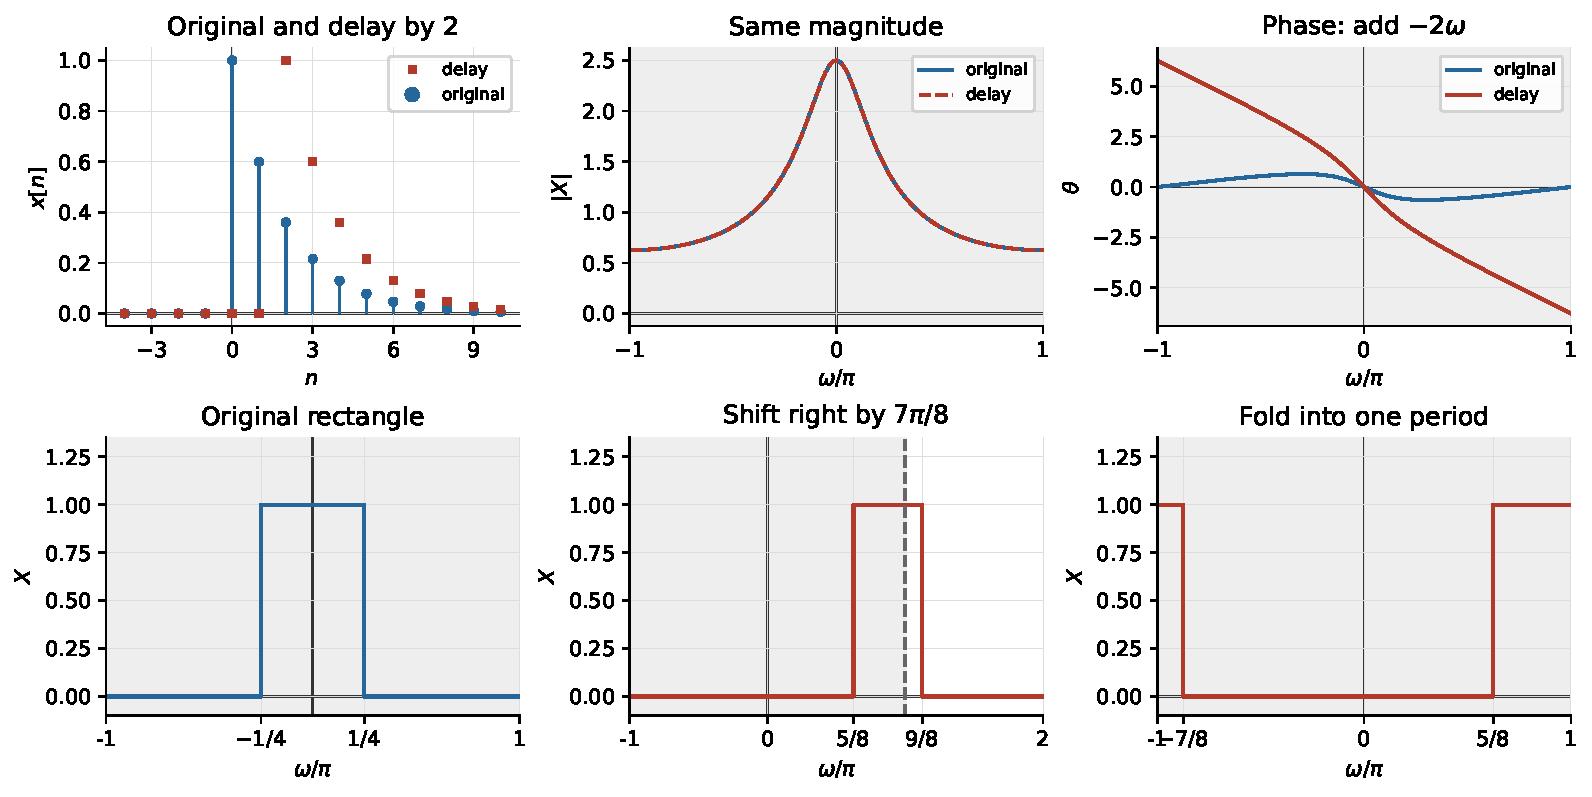
\includegraphics[width=0.96\textwidth]{07-dtft/shifts.pdf}
  \caption{上行：$0.6^n u[n]$ 延迟两个样值，幅度谱相同，相位增加 $-2\omega$。相位按连续分支显示。下行：$R_{\pi/4}$ 右移 $7\pi/8$，跨越 $\pi$ 的部分折回 $-\pi$ 附近。}
  \label{fig:dtft-shifts}
\end{figure}

\subsection{时域差分}
\label{sec:dtft-difference}

利用线性和时移性质，
\begin{equation}
  x[n]-x[n-1]\fourierpair
  (1-\e^{-\iu\omega})X(\e^{\iu\omega}).
  \label{eq:dtft-difference}
\end{equation}
\keyterm{一阶后向差分（first backward difference）}比较当前与前一时刻的样值；频域乘子可写成
\[
  1-\e^{-\iu\omega}
  =2\iu\e^{-\iu\omega/2}\sin\frac{\omega}{2},
  \qquad |1-\e^{-\iu\omega}|=2\left|\sin\frac{\omega}{2}\right|.
\]
它在零频处为零，\red{差分消去常数分量}；在 $\omega=\pi$ 处幅度为 $2$，更强调逐点交替的分量。这个乘子的\red{幅度并非正比于全频率}，只在零频附近有 $1-\e^{-\iu\omega}\approx\iu\omega$，可与连续时间求导的乘子 $\iu\omega$ 对照。

对 $x[n]=\stepfun[n]$，时域差分为 $\impulse[n]$。频域上，分式乘以 $1-\e^{-\iu\omega}$ 后为 $1$，而周期冲激项被零点消去，结果与 $\impulse[n]\fourierpair1$ 一致。

\subsection{时域扩展与插零}
\label{sec:dtft-expansion}

离散序列仅在整数下标有定义。取正整数 $k$，\keyterm{时域扩展（time expansion）}定义为
\begin{equation}
  x_{(k)}[n]=
  \begin{cases}
    x[n/k],&n\text{ 是 }k\text{ 的整数倍},\\
    0,&\text{其他}.
  \end{cases}
  \label{eq:dtft-expansion-definition}
\end{equation}
它在相邻样值间\red{插入指定数量的零}，零样值个数为 $k-1$；原来位于 $m$ 的样值移到 $km$。只对非零位置求和，
\[
  X_{(k)}(\e^{\iu\omega})
  =\sum_m x_{(k)}[km]\e^{-\iu\omega km}
  =\sum_m x[m]\e^{-\iu(k\omega)m}
  =X(\e^{\iu k\omega}).
\]
所以
\begin{equation}
  \boxed{x_{(k)}[n]\fourierpair X(\e^{\iu k\omega})}.
  \label{eq:dtft-expansion}
\end{equation}
频谱沿频率轴压缩，$2\pi/k$ 成为它的一个周期；一个 $2\pi$ 区间内包含 $k$ 份压缩后的副本。\red{插零不带幅度系数}，因为求和只是重新标记整数位置。连续缩放 $x(t/k)$ 的变换为 $kX(\iu k\Omega)$，其系数来自积分变量代换；这里没有该积分步骤。

\begin{example}[五点矩形插一个零]
  记 $v[n]=\mathbf1_{|n|\le2}$，则 $v_{(2)}[n]$ 仅在 $n=-4,-2,0,2,4$ 处取 $1$，其余位置均为零。由\cref{eq:dtft-rectangle}，
  \[
    V(\e^{\iu\omega})=\frac{\sin(5\omega/2)}{\sin(\omega/2)},
    \qquad
    V_{(2)}(\e^{\iu\omega})
      =V(\e^{2\iu\omega})=\frac{\sin(5\omega)}{\sin\omega}.
  \]
  后者以 $\pi$ 为周期，在所有 $\omega=m\pi$ 处均须补值 $5$。时域图须保留相邻非零样值间的零位置，见\cref{fig:dtft-expansion}。
  \begin{figure}[H]
    \centering
    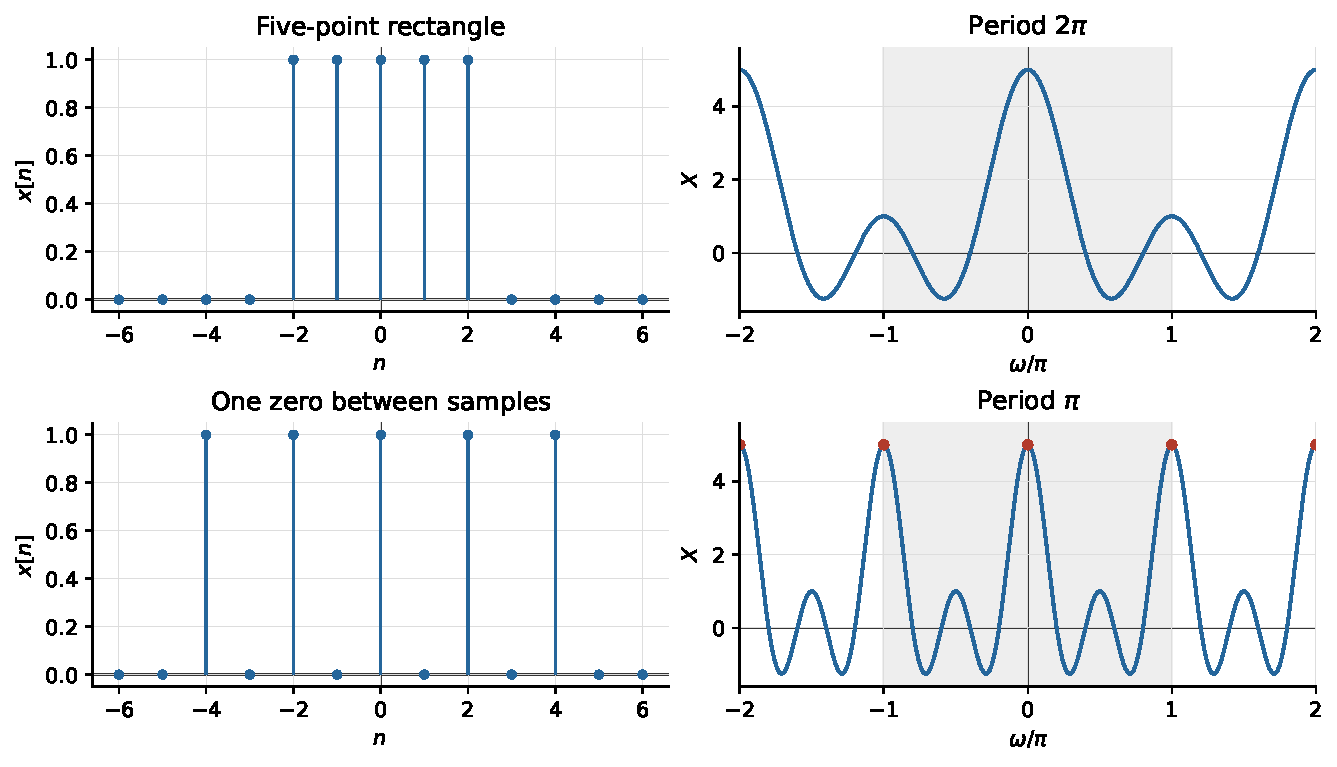
\includegraphics[width=0.92\textwidth]{07-dtft/expansion.pdf}
    \caption{五点矩形插零前后。样值的位置间距加倍，带符号频谱压缩并重复，峰值仍为 $5$。}
    \label{fig:dtft-expansion}
  \end{figure}
\end{example}

\begin{pitfall}[把插零当作任意尺度变换]
  $x[n/k]$ 在非整数自变量处没有定义，必须连同\cref{eq:dtft-expansion-definition} 的零值分支一起使用。$x[kn]$ 则只保留每隔 $k$ 个位置的样值，是另一种运算；不能由插零公式把 $k$ 换成 $1/k$ 来求其频谱。
\end{pitfall}

\subsection{频域微分与多项式加权指数}
\label{sec:dtft-frequency-derivative}

若 $\sum_n(1+|n|)|x[n]|<\infty$，可逐项求导：
\[
  \frac{\dd X(\e^{\iu\omega})}{\dd\omega}
  =\sum_n(-\iu n)x[n]\e^{-\iu\omega n}.
\]
乘以 $\iu$，得到
\begin{equation}
  \boxed{n x[n]\fourierpair
    \iu\frac{\dd X(\e^{\iu\omega})}{\dd\omega}}.
  \label{eq:dtft-frequency-derivative}
\end{equation}
该条件是\blue{保证普通求导成立的充分条件}；在分布意义下，频域导数也可另行定义。\red{时域乘下标对应频域求导}，与连续时间的 $t x(t)\fourierpair\iu\,\dd X/\dd\omega$ 具有相同形式。符号检查要保留求导产生的 $-\iu n$，再乘 $\iu$。

对 $|a|<1$，从\cref{eq:dtft-exponential} 出发，
\begin{align*}
  n a^n\stepfun[n]
    &\fourierpair
      \iu\frac{\dd}{\dd\omega}\frac1{1-a\e^{-\iu\omega}}
      =\frac{a\e^{-\iu\omega}}{(1-a\e^{-\iu\omega})^2},\\
  (n+1)a^n\stepfun[n]
    &\fourierpair
      \frac{a\e^{-\iu\omega}}{(1-a\e^{-\iu\omega})^2}
      +\frac{1-a\e^{-\iu\omega}}{(1-a\e^{-\iu\omega})^2}
      =\frac1{(1-a\e^{-\iu\omega})^2}.
\end{align*}
更一般地，取正整数 $r$，定义
\[
  p_{r,a}[n]=
  \begin{cases}
    \displaystyle\binom{n+r-1}{r-1}a^n,&n\ge0,\\
    0,&n<0.
  \end{cases}
\]
由二项级数 $(1-z)^{-r}=\sum_{n=0}^{\infty}\binom{n+r-1}{r-1}z^n$（$|z|<1$），
\begin{equation}
  \boxed{p_{r,a}[n]\fourierpair
    \frac1{(1-a\e^{-\iu\omega})^r}},\qquad |a|<1.
  \label{eq:dtft-repeated-pole}
\end{equation}
其中 $\binom{n+r-1}{r-1}=(n+r-1)!/[n!(r-1)!]$ 只在 $n\ge0$ 分支使用。$r=1$ 是指数，$r=2$ 是 $(n+1)a^n$，$r=3$ 是 $(n+1)(n+2)a^n/2$；$a=0$ 时均约定零点样值为 $1$，其余为零。\red{高次分母对应多项式因子}，反演时不能把分母次数当作指数参数的幂次。$r=2$ 的样值与幅相谱见\cref{fig:dtft-weighted-exponential}。
\begin{figure}[H]
  \centering
  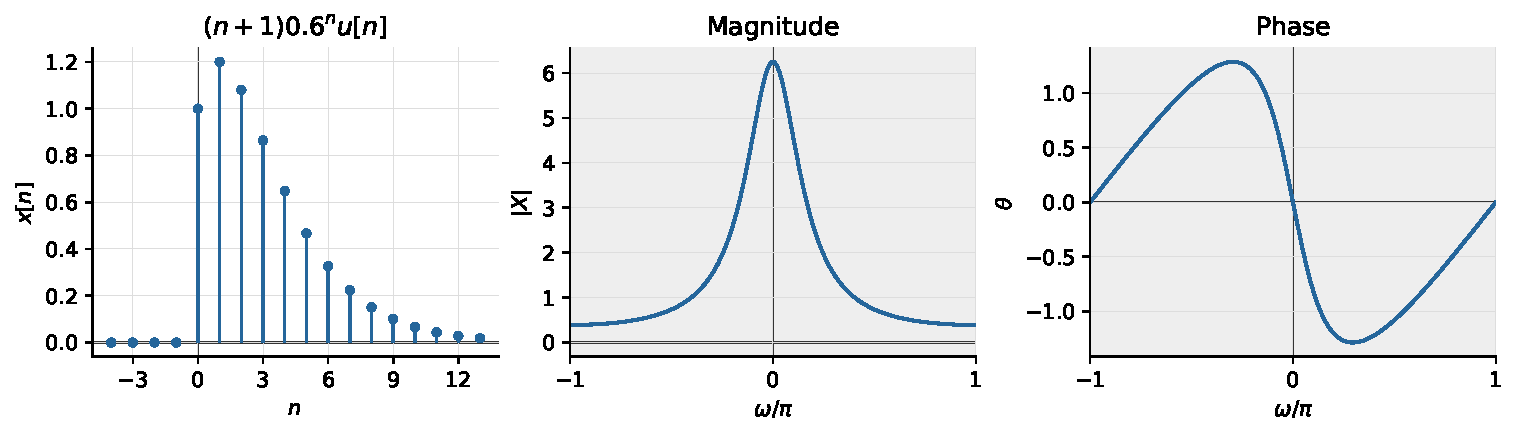
\includegraphics[width=0.96\textwidth]{07-dtft/weighted-exponential.pdf}
  \caption{$(n+1)0.6^n u[n]$ 及其幅相谱。频谱为 $(1-0.6e^{-\iu\omega})^{-2}$；相位按连续分支显示。}
  \label{fig:dtft-weighted-exponential}
\end{figure}

\subsection{时域卷积性质}
\label{sec:dtft-convolution}

若 $x[n]$ 与 $h[n]$ 绝对可和，卷积也绝对可和，并有
\begin{equation}
  \boxed{x[n]\conv h[n]\fourierpair
    X(\e^{\iu\omega})H(\e^{\iu\omega})}.
  \label{eq:dtft-convolution}
\end{equation}
为证明该式，把卷积和代入定义，交换两次求和，再令 $m=n-k$：
\begin{align*}
  Y(\e^{\iu\omega})
    &=\sum_n\left[\sum_k x[k]h[n-k]\right]\e^{-\iu\omega n}\\
    &=\sum_k x[k]\e^{-\iu\omega k}
      \sum_n h[n-k]\e^{-\iu\omega(n-k)}\\
    &=\left[\sum_k x[k]\e^{-\iu\omega k}\right]
      \left[\sum_m h[m]\e^{-\iu\omega m}\right]
      =X(\e^{\iu\omega})H(\e^{\iu\omega}).
\end{align*}
这一步把\red{卷积和变成普通乘法}。与逆变换不同，此处\red{乘积没有归一化系数}，不额外乘 $1/(2\pi)$。含阶跃或正弦等广义频谱时，还须确认时域卷积与频域乘积有定义，\blue{不能任意相乘两个奇异分布}。

\subsection{时域累加性质}
\label{sec:dtft-accumulation}

令
\[
  y[n]=\sum_{k=-\infty}^{n}x[k]=x[n]\conv\stepfun[n].
\]
先假设 $\sum_n(1+|n|)|x[n]|<\infty$，从而各个累加值存在，且 $X$ 可微。将阶跃频谱代入卷积性质，并在冲激处取样：
\begin{align*}
  Y(\e^{\iu\omega})
    &=X(\e^{\iu\omega})\left[
        \operatorname{pv}\frac1{1-\e^{-\iu\omega}}
        +\pi\sum_m\impulse(\omega-2m\pi)\right]\\
    &=\operatorname{pv}\frac{X(\e^{\iu\omega})}{1-\e^{-\iu\omega}}
        +\pi X(\e^{\iu0})\sum_m\impulse(\omega-2m\pi).
\end{align*}
这里 $X(\e^{\iu0})=\sum_n x[n]$，周期性保证所有 $\omega=2m\pi$ 处的取样值相同。故
\begin{equation}
  \boxed{\sum_{k=-\infty}^{n}x[k]\fourierpair
    \operatorname{pv}\frac{X(\e^{\iu\omega})}{1-\e^{-\iu\omega}}
    +\pi X(\e^{\iu0})\sum_m\impulse(\omega-2m\pi)}.
  \label{eq:dtft-accumulation}
\end{equation}
即使输入有限长，累加结果也可能在右端保持常数，所以输出频谱须按广义函数理解。\red{累加须保留直流冲激}；\blue{输入全部样值之和为零时}，这个冲激项才消失。

从 $y[n]-y[n-1]=x[n]$ 只能得到
$(1-\e^{-\iu\omega})Y=X$。由于差分会消去常数，直接除以 $1-\e^{-\iu\omega}$ 会丢失有关累加常数的信息。\red{差分不能确定累加常数}，这里由求和下限 $-\infty$ 选定左端累加值为零。

还可把主值项单独解释为
\begin{equation}
  \stepfun[n]-\frac12\fourierpair
  \operatorname{pv}\frac1{1-\e^{-\iu\omega}}.
  \label{eq:dtft-step-without-dc}
\end{equation}
常数 $1/2$ 的频谱恰为 $\pi\sum_m\impulse(\omega-2m\pi)$。因此
\[
  x\conv\left(\stepfun-\frac12\right)
  =\sum_{k=-\infty}^{n}x[k]-\frac12\sum_k x[k].
\]
只有主值分式的反演与真正的累加相差一个常数。五点矩形的逐项计算见\cref{ex:dtft-principal-sum}。

\section{离散 LTI 系统的频率响应}
\label{sec:dtft-lti}

\subsection{由单位脉冲响应到频率响应}

对单位脉冲响应为 $h[n]$ 的离散 LTI 系统，
\[
  x[n]\longrightarrow\boxed{h[n]}\longrightarrow
  y[n]=x[n]\conv h[n].
\]
频率响应（frequency response）为
\begin{equation}
  H(\e^{\iu\omega})=\sum_n h[n]\e^{-\iu\omega n},
  \qquad Y(\e^{\iu\omega})=H(\e^{\iu\omega})X(\e^{\iu\omega}).
  \label{eq:dtft-lti-response}
\end{equation}
它是\red{单位脉冲响应的变换}。$|H|$ 给出各频率的幅度增益，$\arg H$ 给出相位变化；对普通非零频谱，
\[
  |Y|=|H||X|,\qquad
  \arg Y=\arg H+\arg X\pmod{2\pi}.
\]
零点处不使用相位相加式。若 $H$ 和 $Y$ 可由已知输入输出求出，形式上有 $H=Y/X$，但\red{只能在输入频谱非零处相除}；输入没有激励到的频率，通常不能仅凭该组输入输出确定响应。\cref{ex:dtft-identify-system} 给出输入频谱处处非零的情况。

若 $\sum_n|h[n]|<\infty$，$H$ 为普通连续函数，系统 BIBO 稳定；\blue{因果还须另查} $h[n]=0$（$n<0$），两条时域判据见第四章。以广义函数形式写出 $H$，不自动保证稳定性。

\subsection{差分器、累加器与延时器}
\label{sec:dtft-elementary-systems}

差分器由 $y[n]=x[n]-x[n-1]$ 定义，输入单位脉冲即得
\[
  h[n]=\impulse[n]-\impulse[n-1],\qquad
  H(\e^{\iu\omega})=1-\e^{-\iu\omega}.
\]
它有两个非零脉冲响应样值，绝对可和；幅度在零频处为零、在 $\pi$ 处为 $2$，与\cref{sec:dtft-difference} 一致。\red{差分器抑制低频}，幅度图见\cref{fig:dtft-elementary-systems}。

累加器的零状态关系是
\[
  y[n]=\sum_{k=-\infty}^{n}x[k],\qquad h[n]=\stepfun[n],
\]
故由\cref{eq:dtft-step}，
\[
  H(\e^{\iu\omega})
  =\operatorname{pv}\frac1{1-\e^{-\iu\omega}}
    +\pi\sum_m\impulse(\omega-2m\pi).
\]
它因果，但 $h[n]$ \blue{不绝对可和}，\red{累加器不满足稳定判据}。例如从零时刻开始的有界阶跃输入产生
$(n+1)\stepfun[n]$，输出无界。含奇点与冲激的频谱不能当作零频处取有限值的普通频率响应。

对整数 $n_0$，延时器为
\[
  y[n]=x[n-n_0],\qquad
  h[n]=\impulse[n-n_0],\qquad
  H(\e^{\iu\omega})=\e^{-\iu\omega n_0}.
\]
其幅度处处为 $1$，相位可取 $-\omega n_0$；\red{纯延时只改变相位}。系统稳定，$n_0\ge0$ 时因果；$n_0<0$ 时是超前器。
\begin{figure}[H]
  \centering
  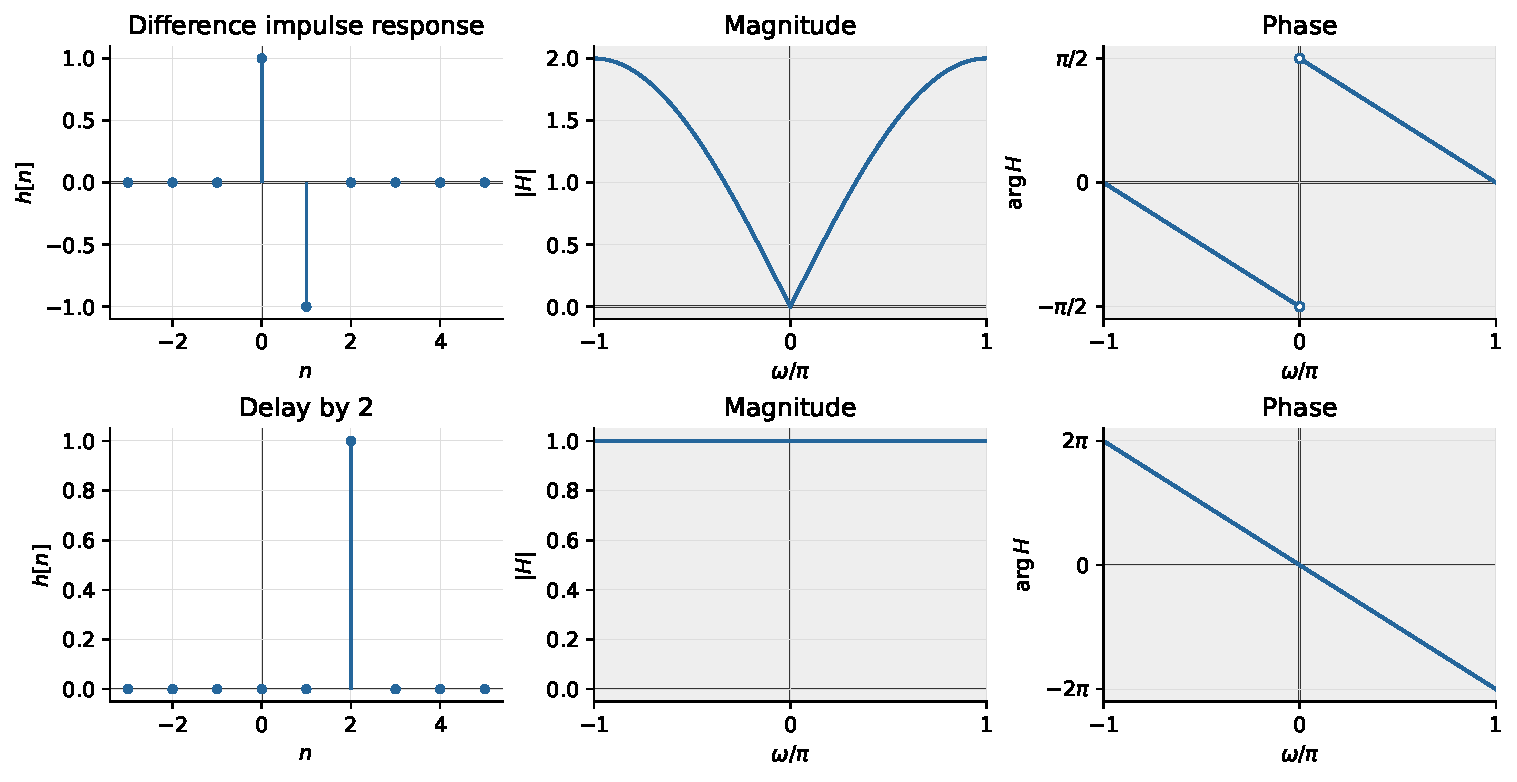
\includegraphics[width=0.94\textwidth]{07-dtft/elementary-systems.pdf}
  \caption{差分器与两样值延时器的脉冲响应和幅相特性。差分器在零频处相位未定义；延时器的相位按连续分支显示。累加器的广义频谱见\cref{fig:dtft-step}。}
  \label{fig:dtft-elementary-systems}
\end{figure}

\subsection{复指数与余弦输入的响应}
\label{sec:dtft-sinusoidal-response}

若 $h[n]$ 绝对可和，对输入 $\e^{\iu\omega_0n}$，
\[
  y[n]=\sum_k h[k]\e^{\iu\omega_0(n-k)}
    =\e^{\iu\omega_0n}\sum_k h[k]\e^{-\iu\omega_0k}
    =H(\e^{\iu\omega_0})\e^{\iu\omega_0n}.
\]
因此复指数经过 LTI 系统后\red{频率保持不变}，只乘以该频率处的复增益。这里输入在所有整数时刻存在；若乘上 $\stepfun[n]$ 使其从零时刻开始，完整输出还可能含有起始过程，\blue{不能直接套这个式子}。

对 $x[n]=\cos(\omega_0n)$，先取 $0<\omega_0<\pi$，一个主周期内有 $\pm\omega_0$ 两条权重为 $\pi$ 的谱线。频域乘以 $H$，利用冲激取样，
\begin{align*}
  Y(\e^{\iu\omega})
    &=\pi H(\e^{\iu\omega_0})\sum_m
       \impulse(\omega-\omega_0-2m\pi)\\
    &\quad+\pi H(\e^{-\iu\omega_0})\sum_m
       \impulse(\omega+\omega_0-2m\pi).
\end{align*}
每条谱线的位置不变，权重乘以相应的 $H$，如\cref{fig:dtft-sinusoidal-response}。反演时，每条权重须除以 $2\pi$，故
\begin{equation}
  y[n]=\frac12\left[
    H(\e^{\iu\omega_0})\e^{\iu\omega_0n}
    +H(\e^{-\iu\omega_0})\e^{-\iu\omega_0n}\right].
  \label{eq:dtft-cosine-response-general}
\end{equation}
若 $h[n]$ 为实序列，求和取共轭即得
$H(\e^{-\iu\omega_0})=H^*(\e^{\iu\omega_0})$。两项才能合成实余弦：
\begin{equation}
  \boxed{y[n]=|H(\e^{\iu\omega_0})|
    \cos\bigl(\omega_0n+\arg H(\e^{\iu\omega_0})\bigr)}.
  \label{eq:dtft-cosine-response-real}
\end{equation}
\red{合成实余弦须检查实系统}；一般复值 $h$ 应保留\cref{eq:dtft-cosine-response-general}。若 $H(\e^{\iu\omega_0})=0$，实系统的输出为零，不再指定相位。$\omega_0=0$ 或 $\pi$ 时两组谱线重合，应先合并权重，按单个复指数处理。
\begin{figure}[H]
  \centering
  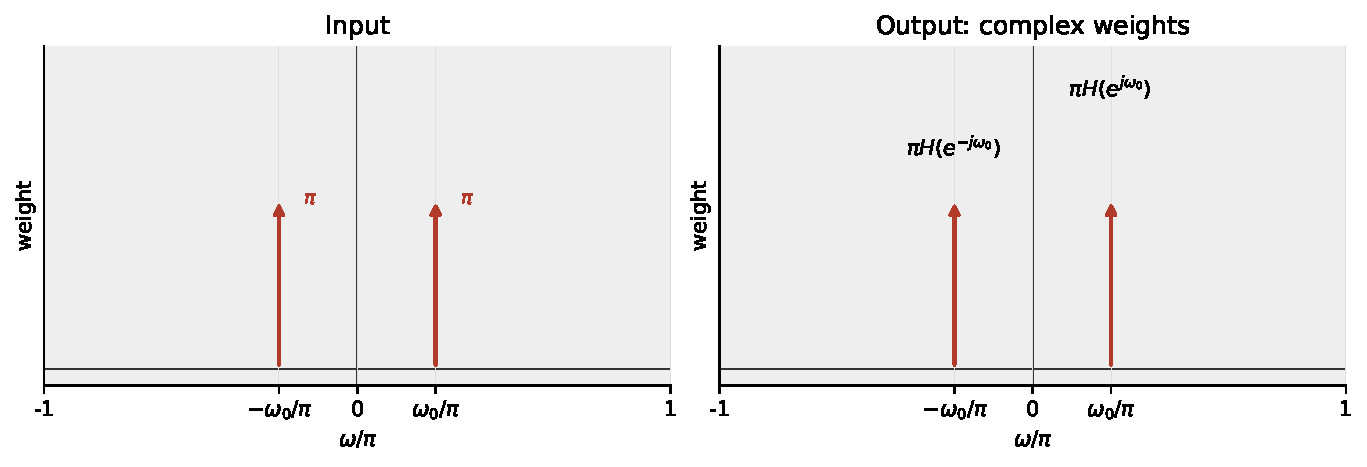
\includegraphics[width=0.94\textwidth]{07-dtft/sinusoidal-response.pdf}
  \caption{余弦通过实系数 LTI 系统：两条输入谱线分别乘以相应的复增益。箭头仅标谱线位置与权重，竖向长度不表示有限的频谱高度；两条输出权重互为共轭。}
  \label{fig:dtft-sinusoidal-response}
\end{figure}

\subsection{由常系数差分方程求响应}
\label{sec:dtft-difference-equation}

设零状态 LTI 系统满足\keyterm{常系数差分方程（linear constant-coefficient difference equation）}
\[
  \sum_{k=0}^{N}a_k y[n-k]=\sum_{k=0}^{M}b_k x[n-k].
\]
用时移性质逐项变换，
\[
  \left[\sum_{k=0}^{N}a_k\e^{-\iu\omega k}\right]Y(\e^{\iu\omega})
  =\left[\sum_{k=0}^{M}b_k\e^{-\iu\omega k}\right]X(\e^{\iu\omega}).
\]
在分母非零且普通频率响应存在时，
\begin{equation}
  H(\e^{\iu\omega})
  =\frac{\displaystyle\sum_{k=0}^{M}b_k\e^{-\iu\omega k}}
         {\displaystyle\sum_{k=0}^{N}a_k\e^{-\iu\omega k}}.
  \label{eq:dtft-difference-equation}
\end{equation}
求解时\red{先说明零状态条件}。给定差分方程还可能有不同的齐次解；因果性、初始条件或稳定性用于选定所讨论的系统。带独立初始储能的总响应不能直接写成 $Y=HX$。

课程计算可按以下顺序进行：
\begin{enumerate}
  \item 每个延迟 $k$ 写成乘子 $\e^{-\iu\omega k}$，移项后提取 $Y$ 与 $X$。
  \item 分母按 $\e^{-\iu\omega}$ 因式分解，再展开部分分式。
  \item 不同的一次因子用\cref{eq:dtft-exponential} 反演；重复因子用\cref{eq:dtft-repeated-pole}。
  \item 求输出时再乘输入频谱，检查输入是否使一次因子变成重复因子。
\end{enumerate}
\red{输出可能新增重复因子}，不能沿用求 $h[n]$ 时的部分分式形式。完整计算见\cref{ex:dtft-difference-equation}；若所得右侧指数参数的模不小于 $1$，\blue{还须回查 DTFT 的收敛条件}。

\section{调制性质与频域周期卷积}
\label{sec:dtft-modulation}

\subsection{时域相乘与一个周期内的卷积}

设 $x[n]\fourierpair X(\e^{\iu\omega})$、$y[n]\fourierpair Y(\e^{\iu\omega})$，时域乘积为 $z[n]=x[n]y[n]$。两个频谱均以 $2\pi$ 为周期，定义其\keyterm{周期卷积（periodic convolution）}
\[
  (X*_{2\pi}Y)(\omega)
    =\int_{\alpha}^{\alpha+2\pi}
       X(\e^{\iu\theta})Y(\e^{\iu(\omega-\theta)})\dd\theta.
\]
被积函数对 $\theta$ 也以 $2\pi$ 为周期，故结果与起点 $\alpha$ 无关。调制性质为
\begin{equation}
  \boxed{x[n]y[n]\fourierpair
    \frac1{2\pi}(X*_{2\pi}Y)(\omega)}.
  \label{eq:dtft-multiplication}
\end{equation}
这里的星号表示\red{只积一个周期的卷积}；须保留\red{归一化系数} $1/(2\pi)$。

先在两个序列都绝对可和的条件下证明。将 $x[n]$ 写成逆变换，交换求和与积分：
\begin{align*}
  Z(\e^{\iu\omega})
    &=\sum_n y[n]\e^{-\iu\omega n}
        \frac1{2\pi}\int_{\alpha}^{\alpha+2\pi}
          X(\e^{\iu\theta})\e^{\iu\theta n}\dd\theta\\
    &=\frac1{2\pi}\int_{\alpha}^{\alpha+2\pi}
        X(\e^{\iu\theta})
        \left[\sum_n y[n]\e^{-\iu(\omega-\theta)n}\right]\dd\theta\\
    &=\frac1{2\pi}\int_{\alpha}^{\alpha+2\pi}
        X(\e^{\iu\theta})Y(\e^{\iu(\omega-\theta)})\dd\theta.
\end{align*}
\blue{对两个有限能量序列}，该式也成立：时域乘积绝对可和，频域周期卷积可由平方可积频谱定义，并用有限截断的极限得到。

与\cref{eq:dtft-convolution} 对照，时域卷积对应频谱的普通乘法，没有 $1/(2\pi)$；时域乘法对应频谱的周期卷积，带 $1/(2\pi)$。连续时间的调制性质见\cref{eq:ctft-frequency-convolution}，其频域卷积在整条实轴上积分。两个非零周期频谱不能直接在整条实轴上做普通卷积，否则\red{会重复计算所有副本}，积分通常发散。

\subsection{先做普通卷积，再周期叠加}
\label{sec:dtft-periodic-folding}

作图时可截取两个频谱在 $[-\pi,\pi)$ 的一份，分别记作 $X_0(\omega)$、$Y_0(\omega)$，区间外取零。先算普通卷积
\[
  C_0(\omega)=\int_{-\infty}^{\infty}
        X_0(\theta)Y_0(\omega-\theta)\dd\theta,
\]
再将结果以 $2\pi$ 为间隔平移相加：
\begin{equation}
  Z(\e^{\iu\omega})=\frac1{2\pi}
      \sum_{m=-\infty}^{\infty}C_0(\omega-2m\pi).
  \label{eq:dtft-periodic-folding}
\end{equation}
计算顺序是：\hl{先卷积，再周期平移}；\hl{重合部分逐点相加}。折回主周期\red{会同时带入相邻副本}，不能只把中央曲线截在 $[-\pi,\pi)$ 内。

例如两个高度为 $1$、支撑为 $(-a,a)$ 的矩形相卷积，在 $\omega$ 处的值是区间 $(-a,a)$ 与 $(\omega-a,\omega+a)$ 的重叠长度：
\[
  C_0(\omega)=(2a-|\omega|)_+,\qquad
  (v)_+=\max(v,0).
\]
当 $2a<\pi$ 时，\red{中央三角形落在主周期内部}；当 $2a>\pi$ 时，相邻三角形进入主周期，必须叠加。\cref{ex:dtft-sinc-square-wide} 给出宽矩形的分段计算和另一种时域解法。

\subsection{余弦调制与低通、高通的转换}

用欧拉公式和\cref{eq:dtft-frequency-shift}，直接得到
\begin{equation}
  x[n]\cos(\omega_0n)\fourierpair
  \frac12\left[
    X(\e^{\iu(\omega-\omega_0)})
    +X(\e^{\iu(\omega+\omega_0)})\right].
  \label{eq:dtft-cosine-modulation}
\end{equation}
两份频谱分别左右平移，各带系数 $1/2$，越过主周期边界后周期折回，如\cref{fig:dtft-cosine-modulation}。\red{副本重叠时仍须相加}。$\omega_0=\pi$ 时，两份频谱因周期性而相同，得到
\[
  (-1)^nx[n]\fourierpair X(\e^{\iu(\omega-\pi)}).
\]
此时\red{两份半幅合成一份}。低通矩形因此移到 $\pi$ 附近，成为高通；反向再乘一次 $(-1)^n$，即可移回零频。
\begin{figure}[H]
  \centering
  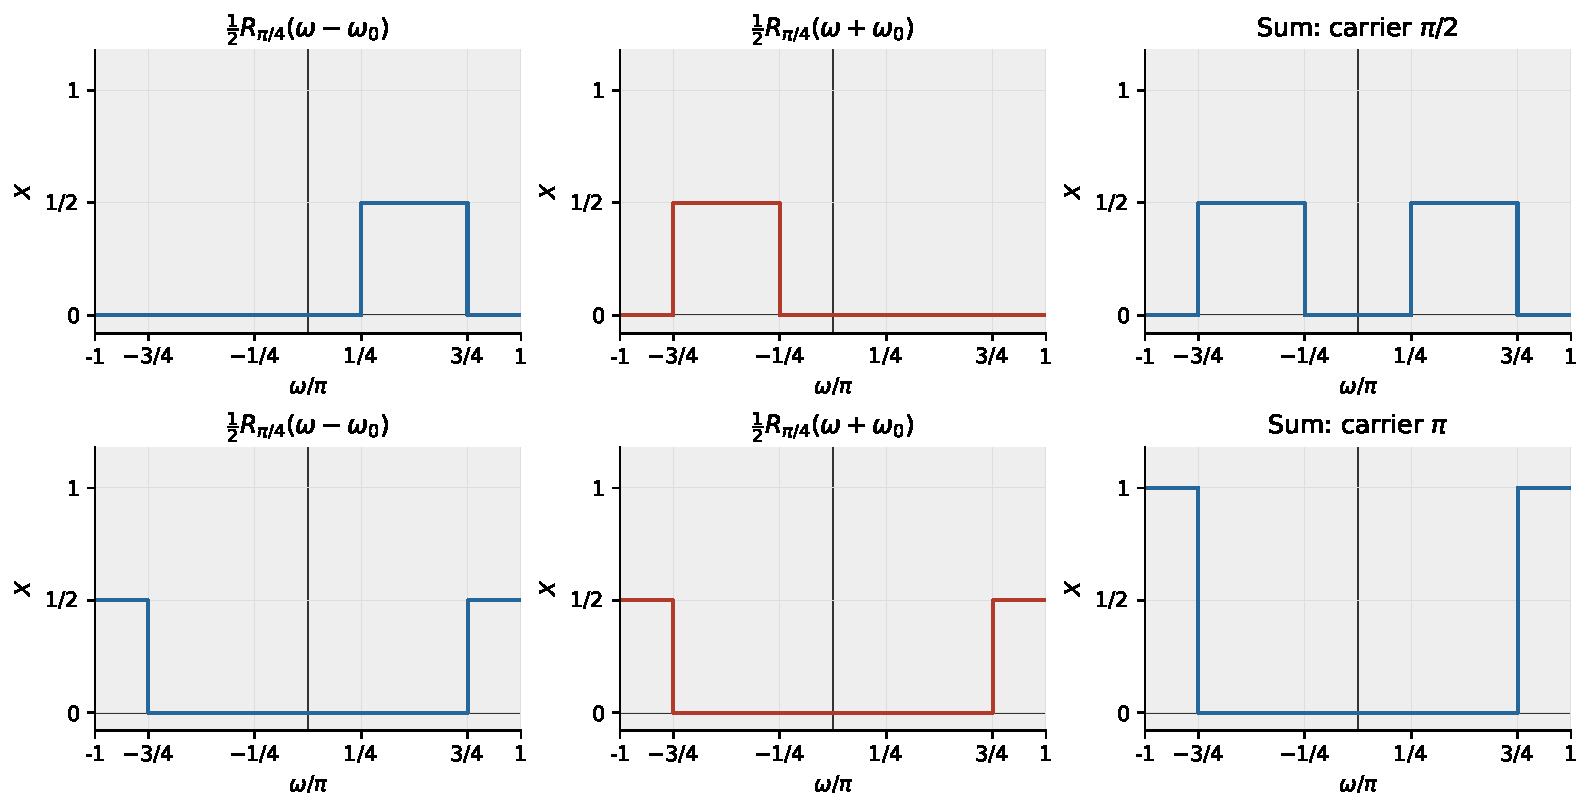
\includegraphics[width=0.94\textwidth]{07-dtft/cosine-modulation.pdf}
  \caption{$R_{\pi/4}$ 的余弦调制。上行载频为 $\pi/2$，产生两份半幅频谱；下行载频为 $\pi$，正负移频副本重合，合成单位高度的高通矩形。}
  \label{fig:dtft-cosine-modulation}
\end{figure}
频移本身不改变矩形形状，所以该低通、高通关系也适用于三角频谱，见\cref{ex:dtft-triangle-inverse}。

\subsection{sinc 平方与周期三角频谱}
\label{sec:dtft-sinc-square}

沿用\cref{sec:dtft-sinc} 的 $s_a[n]=\sin(an)/(\pi n)$、$s_a[0]=a/\pi$，取 $0<a<\pi$。$s_a$ 的频谱为周期矩形，故
\begin{equation}
  \boxed{s_a^2[n]\fourierpair
    \frac1{2\pi}\sum_{m=-\infty}^{\infty}
       (2a-|\omega-2m\pi|)_+}.
  \label{eq:dtft-sinc-square}
\end{equation}
它是\red{三角形的周期叠加}，宽度较大时会带有非零背景；主周期两侧\red{不能只按中央三角形读取}。时域 $n=0$ 处则是\hl{先补值，再平方}，结果为 $a^2/\pi^2$。\cref{ex:dtft-sinc-square-narrow,ex:dtft-sinc-square-wide} 分别计算 $a=\pi/4$ 与 $a=3\pi/4$。

反过来，令 $T_b(\omega)$ 为以 $2\pi$ 为周期、主周期内
\[
  T_b(\omega)=
    \begin{cases}
      1-|\omega|/b,&|\omega|\le b,\\
      0,&b<|\omega|\le\pi,
    \end{cases}
    \qquad 0<b\le\pi.
\]
把上式取 $a=b/2$ 的三角形乘以 $\pi/a=2\pi/b$，得到
\begin{equation}
  t_b[n]=
    \begin{cases}
      \displaystyle\frac{2\sin^2(bn/2)}{b\pi n^2},&n\ne0,\\[4pt]
      \displaystyle\frac{b}{2\pi},&n=0.
    \end{cases}
    \fourierpair T_b(\omega).
  \label{eq:dtft-triangle-pair}
\end{equation}
峰值为 $1$ 的三角形面积为 $b$，其零点样值正好是面积除以 $2\pi$；此式中的 $b$ 是半宽，不能与矩形卷积前的半宽 $a$ 混用。

\section{帕塞瓦尔定理与共轭对称}
\label{sec:dtft-energy-symmetry}

\subsection{一个周期内的能量积分}
\label{sec:dtft-parseval}

对有限能量序列，\keyterm{帕塞瓦尔定理（Parseval's relation）}给出
\begin{equation}
  \boxed{\sum_{n=-\infty}^{\infty}|x[n]|^2
    =\frac1{2\pi}\int_{\alpha}^{\alpha+2\pi}
       |X(\e^{\iu\omega})|^2\dd\omega}.
  \label{eq:dtft-parseval}
\end{equation}
频谱\red{只积一个完整周期}；它的周期副本描述同一组离散频率，把所有周期的能量加起来会重复计数。被积函数为\red{幅度的平方}，一般复频谱不能直接写成 $X^2$。

对有限长或绝对可和序列，将 $X^*$ 展开，再用逆变换：
\begin{align*}
  \frac1{2\pi}\int_{-\pi}^{\pi}XX^*\dd\omega
    &=\frac1{2\pi}\int_{-\pi}^{\pi}
        X(\e^{\iu\omega})
        \sum_n x^*[n]\e^{\iu\omega n}\dd\omega\\
    &=\sum_n x^*[n]\left[
        \frac1{2\pi}\int_{-\pi}^{\pi}
          X(\e^{\iu\omega})\e^{\iu\omega n}\dd\omega\right]\\
    &=\sum_n x^*[n]x[n]=\sum_n|x[n]|^2.
\end{align*}
一般有限能量序列由有限截断及均方极限推广。\cref{eq:ctft-parseval} 的连续时间版本在整条频率轴积分；这里的归一化系数相同，积分区间不同。

例如 $s_a[n]$ 的频谱是高度 $1$、宽度 $2a$ 的周期矩形，故
\[
  \sum_n s_a^2[n]=\frac{2a}{2\pi}=\frac a\pi,
  \qquad 0<a<\pi.
\]
它也等于\cref{eq:dtft-sinc-square} 的零频值；这一核对同时检查周期卷积的系数。排除 $n=0$ 后，右边须减去 $a^2/\pi^2$，\blue{不能省略零点样值}。

\subsection{共轭、翻转与实序列的频谱}
\label{sec:dtft-conjugate-symmetry}

由定义取共轭，以及令 $m=-n$，分别得到
\begin{equation}
  x^*[n]\fourierpair X^*(\e^{-\iu\omega}),
  \qquad x[-n]\fourierpair X(\e^{-\iu\omega}).
  \label{eq:dtft-conjugation-reversal}
\end{equation}
于是实序列的频谱满足
\begin{equation}
  \boxed{X(\e^{-\iu\omega})=X^*(\e^{\iu\omega})}.
  \label{eq:dtft-conjugate-symmetry}
\end{equation}
在普通或均方变换意义下，这一共轭对称条件也能反过来确定 $x[n]$ 为实序列。

写 $X=A+\iu B$，其中 $A,B$ 为实函数。实序列满足
\[
  A(-\omega)=A(\omega),\qquad B(-\omega)=-B(\omega).
\]
即\red{实部偶，虚部奇}。还可进一步得到
\[
  |X(\e^{-\iu\omega})|=|X(\e^{\iu\omega})|,\qquad
  \arg X(\e^{-\iu\omega})\equiv-\arg X(\e^{\iu\omega})
       \pmod{2\pi}.
\]
幅度为偶函数；相位的奇对称按 $2\pi$ 等价理解。\red{相位须保留分支约定}，在负实轴可选 $\pi$ 或 $-\pi$，零频谱处没有相位。$\omega=0,\pi$ 的频谱若有普通函数值，则为实数。

对称性还给出两组常用对应：
\[
  \text{实偶序列}\fourierpair\text{实偶频谱},\qquad
  \text{实奇序列}\fourierpair\text{纯虚奇频谱}.
\]
这些对应\blue{均须保留“实”的条件}。一般复偶序列的频谱仍为偶函数，但未必为实函数。

\subsection{奇偶分量、幅相读取与单侧序列恢复}
\label{sec:dtft-even-odd-recovery}

对于实序列，取
\[
  x_{\mathrm e}[n]=\frac{x[n]+x[-n]}2,\qquad
  x_{\mathrm o}[n]=\frac{x[n]-x[-n]}2.
\]
利用翻转与共轭对称，
\begin{equation}
  \boxed{x_{\mathrm e}[n]\fourierpair\Re X(\e^{\iu\omega}),
  \qquad x_{\mathrm o}[n]\fourierpair\iu\Im X(\e^{\iu\omega})}.
  \label{eq:dtft-even-odd-spectrum}
\end{equation}
因此\red{实部确定偶分量}，\red{虚部确定奇分量}；$\Im X$ 本身不包含前面的 $\iu$，反演奇分量时不能漏掉这个因子。\cref{fig:dtft-even-odd-spectrum} 用一个短实序列展示分解。
\begin{figure}[H]
  \centering
  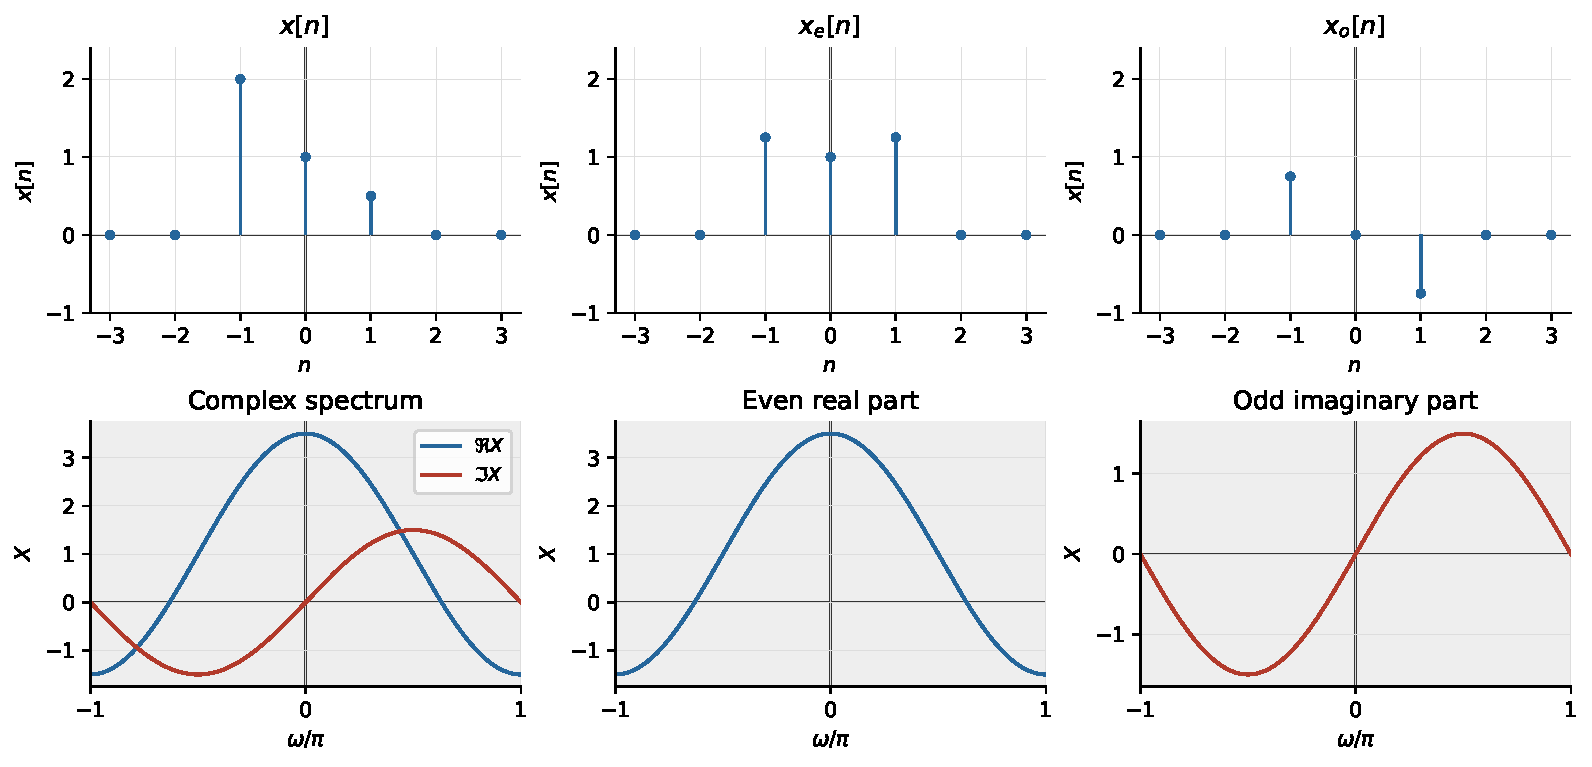
\includegraphics[width=0.96\textwidth]{07-dtft/even-odd-spectrum.pdf}
  \caption{实序列 $x[-1]=2,x[0]=1,x[1]=1/2$ 的奇偶分解。偶分量产生 $1+(5/2)\cos\omega$，奇分量产生 $\iu(3/2)\sin\omega$；底行画频谱的实部或虚部。}
  \label{fig:dtft-even-odd-spectrum}
\end{figure}

读取幅相仍用
\[
  |X|=\sqrt{(\Re X)^2+(\Im X)^2},\qquad
  \arg X=\operatorname{atan2}(\Im X,\Re X),
\]
象限与零点的检查沿用\cref{sec:ctft-magnitude-phase}。只用 $\arctan(\Im X/\Re X)$ \blue{会在负实部区域丢失象限}，也无法处理实部为零的情况。

若另知 $x[n]=0$（$n>0$），则对 $n<0$ 有 $x[-n]=0$，所以 $x[n]=2x_{\mathrm o}[n]$。奇分量的零点恒为零，\blue{不能由虚部确定} $x[0]$；再用能量与零点符号条件可求该样值。频域指数拆分、奇分量作图和能量核对的具体计算见\cref{ex:dtft-imaginary-energy-recovery}。


\section{离散傅里叶级数与有限点 DFT}
\label{sec:dtft-dft}

\subsection{四种傅里叶表示}
\label{sec:fourier-representations}

前面已经分别讨论了连续时间和离散时间的傅里叶表示。按时域对象与频域对象的连续性、离散性，可以作如下区分：
\begin{table}[H]
  \centering
  \caption{四种傅里叶表示的对象和频域形式}
  \label{tab:fourier-representations}
  \begin{tabular}{c c c c}
    \toprule
    表示 & 时域对象 & 频域对象 & 频域形式 \\
    \midrule
    CTFS & 连续时间周期信号 & 离散频率系数 & 离散谱线 \\
    CTFT & 连续时间非周期信号 & 连续频率函数 & 连续频谱 \\
    DTFT & 离散时间序列 & 连续频率函数 & $2\pi$ 周期频谱 \\
    DFT & $N$ 个离散样值 & $N$ 个离散频率样值 & 有限数组 \\
    \bottomrule
  \end{tabular}
\end{table}

表中的 DFT（离散傅里叶变换，discrete Fourier transform）与\keyterm{离散傅里叶级数（discrete-time Fourier series, DTFS）}\red{使用同一组有限维复指数}。若 $x[n]$ 是 $N$ 周期序列，记一个周期内的级数系数为 $a_k$；若只给出 $N$ 个样值并把它们作为有限序列，通常把对应的频域样值记作 $X[k]$。本章采用
\begin{equation}
  X[k]=\sum_{n=0}^{N-1}x[n]\e^{-\iu2\pi kn/N},\qquad
  x[n]=\frac1N\sum_{k=0}^{N-1}X[k]\e^{\iu2\pi kn/N}.
  \label{eq:dft-pair}
\end{equation}
若采用级数的归一化约定
$a_k=N^{-1}\sum_nx[n]\e^{-\iu2\pi kn/N}$，则 $X[k]=Na_k$。这\red{只是归一化位置不同}，复指数基和可恢复的信息相同。

\subsection{从 DTFT 到 DFT}
\label{sec:dtft-to-dft}

设有限序列满足
\[
  x[n]=0,\qquad n\notin\{0,1,\ldots,N-1\}.
\]
它的 DTFT 是有限和
\begin{equation}
  X(\e^{\iu\omega})=\sum_{n=0}^{N-1}x[n]\e^{-\iu\omega n}.
  \label{eq:finite-sequence-dtft}
\end{equation}
在一个完整的 $2\pi$ 周期内取 $N$ 个等间隔频率点
\begin{equation}
  \omega_k=\frac{2\pi k}{N},\qquad k=0,1,\ldots,N-1,
  \label{eq:dft-frequency-grid}
\end{equation}
就得到
\begin{equation}
  X[k]=X(\e^{\iu\omega_k})
  =\sum_{n=0}^{N-1}x[n]\e^{-\iu2\pi kn/N}.
  \label{eq:dft-from-dtft}
\end{equation}
因此
\[
  \Delta\omega=\frac{2\pi}{N}
\]
是 DFT 的频率采样间隔。\red{DFT 是有限长序列 DTFT 的等间隔采样}；它只保留 $N$ 个频率点，不能把这 $N$ 个数\blue{直接当作连续频谱函数}。

还可以把这 $N$ 个时域样值作周期延拓：
\begin{equation}
  \widetilde{x}[n]=x[n\bmod N],
  \qquad \widetilde{x}[n+N]=\widetilde{x}[n].
  \label{eq:dft-periodic-extension}
\end{equation}
对周期延拓序列作离散傅里叶级数，系数为
\[
  a_k=\frac1N\sum_{n=0}^{N-1}x[n]\e^{-\iu2\pi kn/N}
      =\frac{X[k]}{N}.
\]
有限向量、周期延拓和有限序列的 DTFT 是三个不同对象：前者只有 $N$ 个给定分量，第二个在时域按 $N$ 周期重复，第三个在频率上是连续的 $2\pi$ 周期函数。\red{周期延拓不能无说明地代替有限序列}。

\begin{figure}[H]
  \centering
  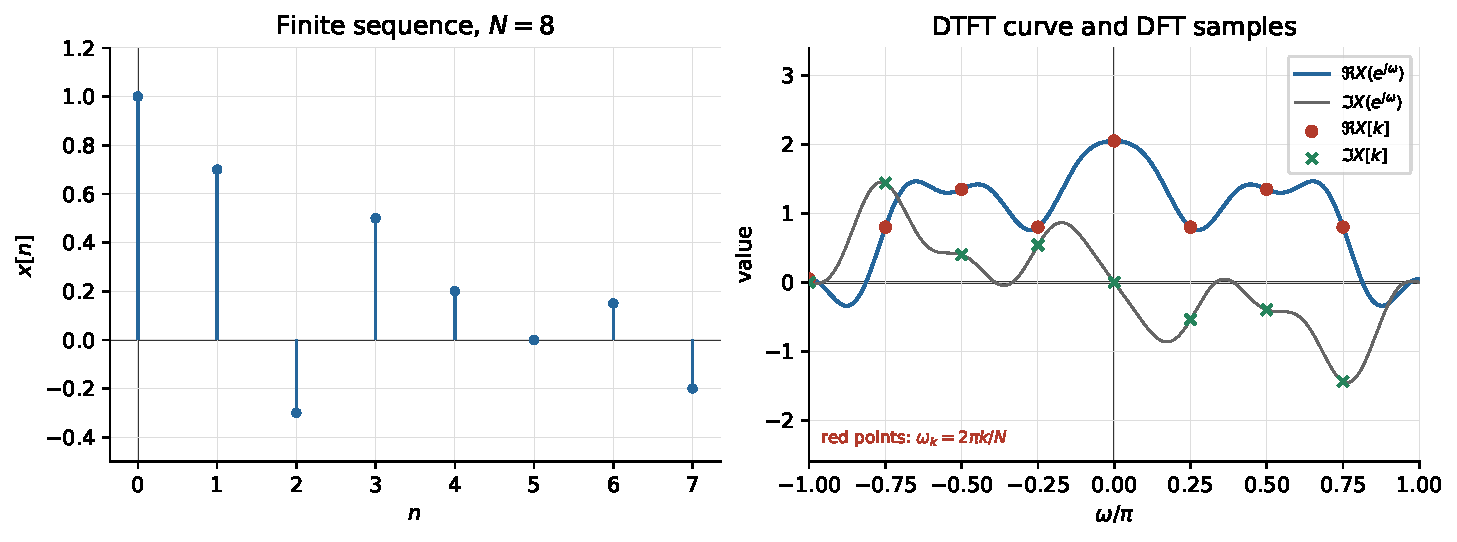
\includegraphics[width=0.94\textwidth]{07-dtft/dft-sampling.pdf}
  \caption{有限长序列的 DTFT 与 DFT 采样点。右图曲线是连续的 $2\pi$ 周期 DTFT，圆点是 $\omega_k=2\pi k/N$ 的 $N$ 个样值，不表示频域冲激谱线。}
  \label{fig:dtft-dft-sampling}
\end{figure}

当频率用 $[-\pi,\pi)$ 的顺序显示时，仍然只有同一组 $N$ 个点。$k>N/2$ 的点可解释为负频率，因为
\[
  \omega_{N-r}=2\pi-\frac{2\pi r}{N}
  \equiv-\frac{2\pi r}{N}\pmod{2\pi}.
\]
公式计算通常按 $k=0,\ldots,N-1$ 排列；中心化显示只改变点的排列顺序。特别地，$\pi$ 和 $-\pi$ 对离散时间复指数是同一个频率。

\subsection{正交性与逆变换}
\label{sec:dft-inverse}

\red{DFT 可逆}的原因是 $N$ 个\red{复指数向量彼此正交}。对 $n,m\in\{0,1,\ldots,N-1\}$，有
\begin{equation}
  \sum_{k=0}^{N-1}\e^{\iu2\pi k(n-m)/N}
  =\begin{cases}
    N,&n=m,\\
    0,&n\ne m.
  \end{cases}
  \label{eq:dft-orthogonality}
\end{equation}
证明时令 $r=\e^{\iu2\pi(n-m)/N}$。当 $n=m$ 时，每一项都是 $1$，和为 $N$。当 $n\ne m$ 时，$r^N=1$ 且 $r\ne1$，故有限等比和为
\[
  \sum_{k=0}^{N-1}r^k=\frac{1-r^N}{1-r}=0.
\]
这里 $|n-m|\le N-1$，所以\blue{分母确实不为零}。

将正变换代入逆变换，得到
\begin{align}
  \frac1N\sum_{k=0}^{N-1}X[k]\e^{\iu2\pi kn/N}
  &=\frac1N\sum_{k=0}^{N-1}
    \left(\sum_{m=0}^{N-1}x[m]\e^{-\iu2\pi km/N}\right)
    \e^{\iu2\pi kn/N}\\
  &=\frac1N\sum_{m=0}^{N-1}x[m]
    \sum_{k=0}^{N-1}\e^{\iu2\pi k(n-m)/N}\\
  =x[n],
  \label{eq:dft-inverse-proof}
\end{align}
其中 $n=0,1,\ldots,N-1$。交换两个有限和后，内层和由正交关系消去所有 $m\ne n$ 的项，只留下 $x[n]$。

\subsection{矩阵表示与下标周期性}
\label{sec:dft-matrix}

定义 DFT 矩阵
\[
  W_{k,n}=\e^{-\iu2\pi kn/N},\qquad k,n=0,1,\ldots,N-1.
\]
令
\[
  \mathbf{x}=[x[0],x[1],\ldots,x[N-1]]^{\mathsf T},\qquad
  \mathbf{X}=[X[0],X[1],\ldots,X[N-1]]^{\mathsf T},
\]
则
\begin{equation}
  \mathbf{X}=\mathbf{W}\mathbf{x},\qquad
  \mathbf{x}=\frac1N\mathbf{W}^{H}\mathbf{X},\qquad
  \mathbf{W}^{-1}=\frac1N\mathbf{W}^{H}.
  \label{eq:dft-matrix}
\end{equation}
矩阵的每一行对应一个频率点，每一列对应一个时域下标；其元素也可写成 $v_k^n$，其中 $v_k=\e^{-\iu2\pi k/N}$。这是一类 Vandermonde 型矩阵。正交关系给出
$\mathbf W^H\mathbf W=N\mathbf I$，所以它的逆矩阵正是 $N^{-1}\mathbf W^H$。

更一般地，若取 $N$ 个两两不同的频率点
$\omega_0,\ldots,\omega_{N-1}$，并令
$v_k=\e^{-\iu\omega_k}$，由有限长序列 DTFT 得到的方程组为
\[
  \begin{bmatrix}
    X(\e^{\iu\omega_0})\\
    X(\e^{\iu\omega_1})\\
    \vdots\\
    X(\e^{\iu\omega_{N-1}})
  \end{bmatrix}
  =
  \begin{bmatrix}
    1&v_0&\cdots&v_0^{N-1}\\
    1&v_1&\cdots&v_1^{N-1}\\
    \vdots&\vdots&&\vdots\\
    1&v_{N-1}&\cdots&v_{N-1}^{N-1}
  \end{bmatrix}
  \begin{bmatrix}
    x[0]\\x[1]\\\vdots\\x[N-1]
  \end{bmatrix}.
\]
这是 Vandermonde 型方程组，其行列式为
\[
  \det\mathbf V
  =\prod_{0\le r<s\le N-1}(v_s-v_r).
\]
由于 $v_0,\ldots,v_{N-1}$ 两两不同，行列式不为零，故矩阵可逆。于是，对时域已知长度为 $N$ 的有限序列，任取 $N$ 个不同频率处的 DTFT 样值，\red{就能恢复全部时域样值} $x[0],\ldots,x[N-1]$，再由有限和式恢复任意 $\omega$ 处的整个 DTFT：
\[
  X(\e^{\iu\omega})
  =\sum_{n=0}^{N-1}x[n]\e^{-\iu\omega n}.
\]
这里的可恢复性依赖于“时域只有 $N$ 个未知样值”这一前提。任意连续频谱函数不能仅凭 $N$ 个点恢复；同时，恢复出整个有限和 DTFT 也不意味着可以把 DFT 数组本身直接当作连续频率函数。

\begin{figure}[H]
  \centering
  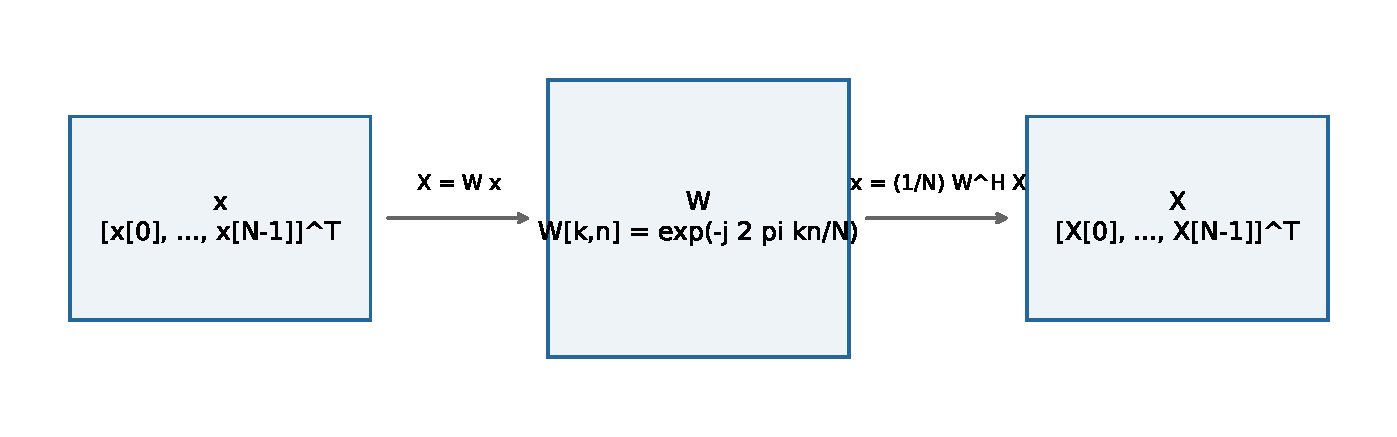
\includegraphics[width=0.86\textwidth]{07-dtft/dft-matrix-flow.pdf}
  \caption{DFT 的有限维线性变换。输入向量由 $N$ 个时域样值组成，经过 DFT 矩阵得到 $N$ 个频域样值。}
  \label{fig:dft-matrix-flow}
\end{figure}

由指数因子的周期性，DFT 下标按 $N$ 周期理解：
\begin{equation}
  X[k+N]=X[k].
  \label{eq:dft-index-periodicity}
\end{equation}
这与 DTFT 的频率周期性
$X(\e^{\iu(\omega+2\pi)})=X(\e^{\iu\omega})$
相互对应，但含义不同：前者是有限数组下标的周期折回，后者是连续频率函数的周期性。计算和存储时保留 $k=0,\ldots,N-1$ 即可；需要负频率显示时，再按模 $N$ 重排。DFT 的 $N$ 个下标是\red{一组完整频率索引}。

\begin{pitfall}
  把 DFT 的 $N$ 个点画成 $N$ 条频域冲激，或把 $X[k]$ 直接当作连续函数，都会混淆 DFT 与 DTFT。\red{DFT 点是频谱样值}；只有常数、正弦等序列的 DTFT 才会在广义函数意义下出现频域冲激串。
\end{pitfall}

\subsection{基 2 快速傅里叶变换}
\label{sec:fft}

直接按定义计算 $N$ 点 DFT 时，每个 $X[k]$ 都要把 $N$ 个时域样值乘上不同的旋转因子再相加，运算量随 $N^2$ 增长。\keyterm{快速傅里叶变换（fast Fourier transform, FFT）}利用复指数的重复关系，把一个 $N$ 点 DFT 拆成两个 $N/2$ 点 DFT，再继续拆分。下面讨论最常用的\keyterm{基 2（radix-2）时间抽取}结构，要求
$N=2^p$。

记
\[
  W_N=\e^{-\iu2\pi/N},\qquad
  X[k]=\sum_{n=0}^{N-1}x[n]W_N^{kn}.
\]
把下标分成偶数和奇数两组：
\[
  E[k]=\sum_{r=0}^{N/2-1}x[2r]W_{N/2}^{kr},\qquad
  O[k]=\sum_{r=0}^{N/2-1}x[2r+1]W_{N/2}^{kr}.
\]
这里 $E[k]$ 是偶下标样值组成的 $N/2$ 点 DFT，$O[k]$ 是奇下标样值组成的 $N/2$ 点 DFT。利用
$W_N^{2kr}=W_{N/2}^{kr}$，可得
\begin{equation}
  X[k]=E[k]+W_N^kO[k],\qquad
  X[k+N/2]=E[k]-W_N^kO[k],
  \quad 0\le k<N/2.
  \label{eq:fft-decimation}
\end{equation}
第二式来自
\[
  W_N^{(k+N/2)(2r+1)}
  =-W_N^{k(2r+1)};
\]
也可以直接使用 $W_N^{k+N/2}=-W_N^k$。因此，两个输出共用同一对较小 DFT，只需先算一次 $W_N^kO[k]$，再分别相加和相减。

\begin{intuition}
  \textbf{蝶形的含义。}
  设上支路输入为 $A$，下支路输入为 $B$，下支路先乘旋转因子 $W$。蝶形输出只有两项：
  \[
    A+WB,\qquad A-WB.
  \]
  图中的两条交叉线表示同一对输入同时送入“加”和“减”两个结果；它们不是额外的信号，也不表示时间上的先后。一个蝶形把两个数变成两个数，信息量没有减少，却\red{把两个输出中重复的计算合并}了。
\end{intuition}

以 $N=8$ 为例，先把
\[
  x[0],x[2],x[4],x[6]
\]
送入一个 $4$ 点 DFT，把
\[
  x[1],x[3],x[5],x[7]
\]
送入另一个 $4$ 点 DFT；再按\cref{eq:fft-decimation} 合并。两个 $4$ 点 DFT 又各自拆成两个 $2$ 点 DFT，$2$ 点 DFT 最后只剩下
\[
  A+B,\qquad A-B,
\]
因为此时旋转因子为 $1$。

\begin{figure}[H]
  \centering
  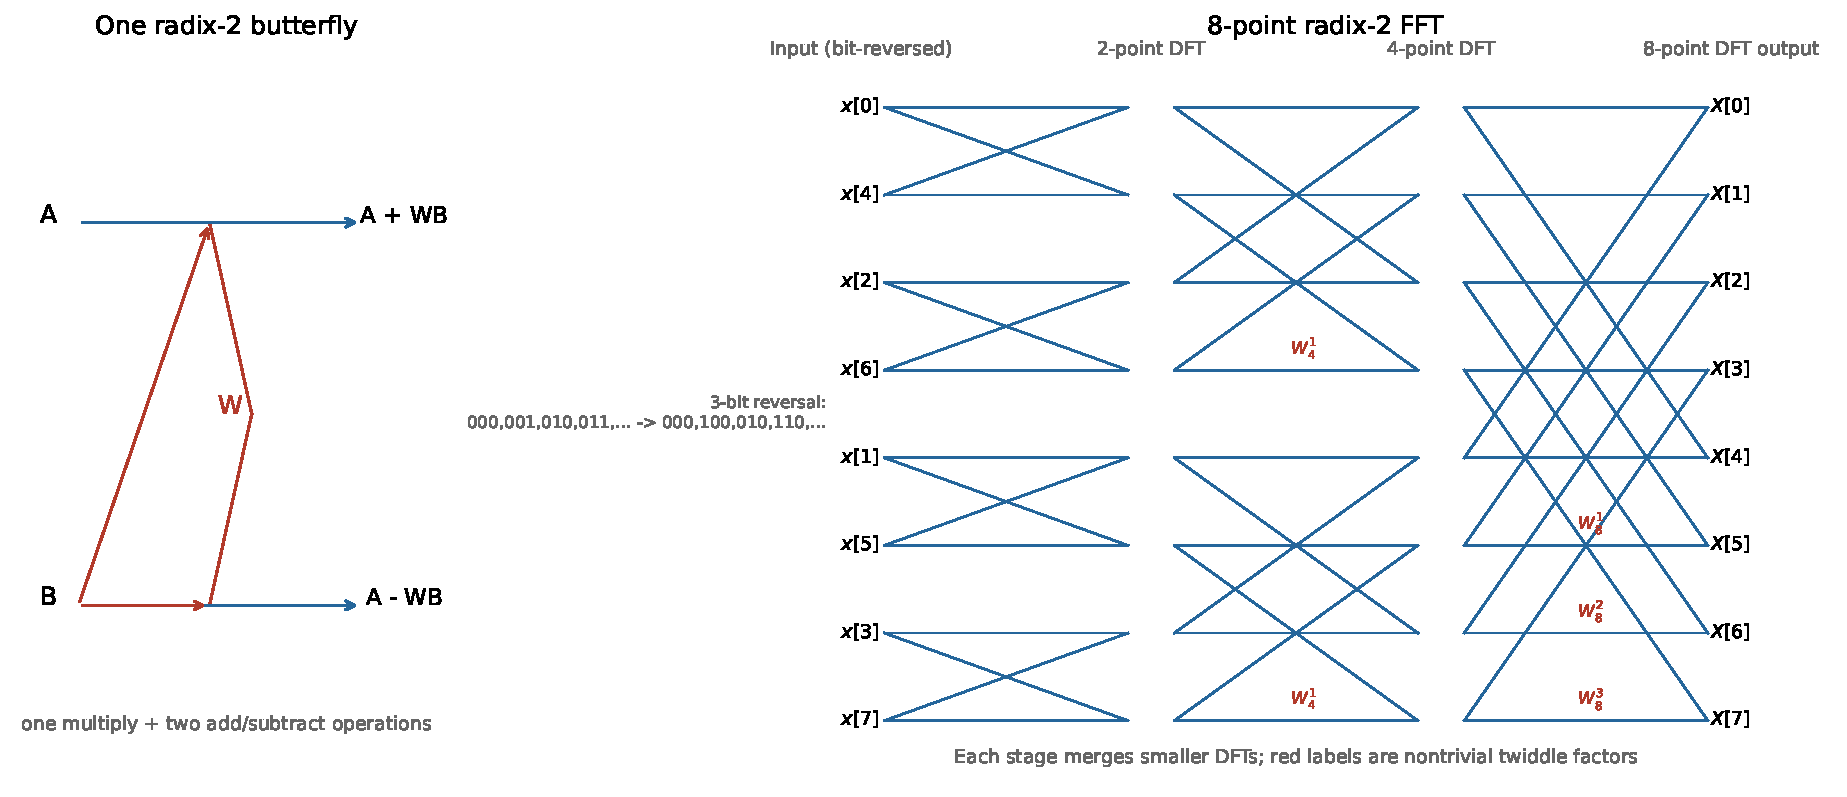
\includegraphics[width=0.98\textwidth]{07-dtft/fft-flow.pdf}
  \caption{基 2 FFT 的流图。左图先说明一个蝶形的两项运算；右图以 8 点 DFT 为例，从位倒序输入开始，依次合并 2 点、4 点和 8 点 DFT。每列的节点是该层已经算出的中间结果，红色因子表示需要乘上的旋转因子。}
  \label{fig:fft-flow}
\end{figure}

\subsubsection{怎样读 8 点 FFT 流图}
\label{sec:fft-flow-reading}

流图应\hl{从左向右读}，每一列代表一次合并：

\begin{enumerate}
  \item 第一列把相邻的两项组成四个 $2$ 点 DFT。每个蝶形只用加法和减法。
  \item 第二列把每两个 $2$ 点结果合成一个 $4$ 点 DFT。这里出现 $W_4^1=-\iu$，所以相应支路要先乘 $-\iu$。
  \item 第三列把两个 $4$ 点结果合成一个 $8$ 点 DFT。四个蝶形分别使用 $W_8^0,W_8^1,W_8^2,W_8^3$；$W_8^0=1$ 的乘法可以省略。
  \item 右端的 $X[0],\ldots,X[7]$ 已按自然下标排列。左端出现
    \[
      x[0],x[4],x[2],x[6],x[1],x[5],x[3],x[7]
    \]
    是因为输入下标先按三位二进制倒序排列。它只是存放顺序的改变，不是把原序列的样值改了。
\end{enumerate}

例如，原下标 $3$ 的二进制写法是 $011$，倒序后为 $110$，对应左端的第 $6$ 个位置，因此 $x[3]$ 出现在 $x[7]$ 后面。按\keyterm{位倒序}后，第一层正好把将在同一个 $2$ 点 DFT 中配对的样值放在相邻位置。若不采用原地流图，也可以保留自然输入顺序，用程序中的索引表完成同样的配对；\red{位倒序是数据排列规则，不是 FFT 的新变换}。

对一般 $N=2^p$，共有 $\log_2N$ 层，每层 $N/2$ 个蝶形，所以蝶形总数为
\[
  \frac{N}{2}\log_2N.
\]
递推关系
\[
  T(N)=2T(N/2)+O(N)
\]
给出
\[
  T(N)=O(N\log_2N).
\]
FFT 的\red{优势来自复指数因子的重复使用}；流图中的同一旋转因子会在许多位置反复出现，不能把每条连线都当成一次全新的 $N$ 项求和。\hl{先看蝶形，再看层数}，\hl{最后数运算量}。

\subsection{循环卷积与 DFT 的乘法性质}
\label{sec:dft-circular-convolution}

普通离散卷积会把两个有限序列的长度相加减一。DFT 的乘法性质对应的是\keyterm{循环卷积}，因为 DFT 把 $N$ 个样值看作一个周期。设 $x[n]$ 和 $h[n]$ 都只给出 $0,\ldots,N-1$ 内的样值，把下标按模 $N$ 折回，定义
\begin{equation}
  y_{\mathrm c}[n]
  =\sum_{m=0}^{N-1}x[m]\,
    h[(n-m)\bmod N],
  \qquad n=0,\ldots,N-1.
  \label{eq:circular-convolution}
\end{equation}
例如 $n=0$ 时，$h[-m]$ 要折回到 $h[(-m)\bmod N]$，所以参与相乘的顺序是
\[
  h[0],h[N-1],h[N-2],\ldots,h[1].
\]
这就是“\hl{先翻转，再按周期平移}”的含义。负下标没有被删掉，而是\red{绕回一个周期的右端}。

\begin{example}
  设
  \[
    x[n]=\{1,2,3,4\},\qquad
    h[n]=\{2,-1,0,1\},
    \qquad 0\le n\le3.
  \]
  循环卷积的四个输出分别为
  \begin{align*}
    y_{\mathrm c}[0]&=1\cdot2+2\cdot1+3\cdot0+4\cdot(-1)=0,\\
    y_{\mathrm c}[1]&=1\cdot(-1)+2\cdot2+3\cdot1+4\cdot0=6,\\
    y_{\mathrm c}[2]&=1\cdot0+2\cdot(-1)+3\cdot2+4\cdot1=8,\\
    y_{\mathrm c}[3]&=1\cdot1+2\cdot0+3\cdot(-1)+4\cdot2=6.
  \end{align*}
  所以
  \[
    y_{\mathrm c}[n]=\{0,6,8,6\}.
  \]
\end{example}

在本例中，普通线性卷积的长度为 $4+4-1=7$。循环卷积只有 $4$ 个输出，线性卷积超过第 $3$ 个下标的部分会绕回前面并与前面的结果相加。对于其他题目，先判断题目要求的\blue{是普通卷积还是循环卷积}；看到模 $N$ 折回，就\red{不能直接套线性卷积的有限支撑范围}。

设 $X[k]$、$H[k]$ 分别是 $x[n]$、$h[n]$ 的 $N$ 点 DFT，$Y_{\mathrm c}[k]$ 是\cref{eq:circular-convolution} 的 DFT。则
\begin{equation}
  Y_{\mathrm c}[k]=X[k]H[k],
  \qquad
  y_{\mathrm c}[n]
  =\frac1N\sum_{k=0}^{N-1}X[k]H[k]\e^{\iu2\pi kn/N}.
  \label{eq:dft-circular-product}
\end{equation}
证明时把 $x[m]$ 与 $h[(n-m)\bmod N]$ 都写成逆 DFT。由于
\[
  \sum_{m=0}^{N-1}\e^{\iu2\pi m(r-s)/N}
  =
  \begin{cases}
    N,&r=s,\\
    0,&r\ne s,
  \end{cases}
\]
不同频率下标的交叉项全部消失，只留下 $X[k]H[k]$。因此，时域的循环卷积在 DFT 域中变成逐点乘法；逆 DFT 再把乘积恢复为一个周期内的 $N$ 个输出样值。

\subsection{用 FFT 计算线性卷积}
\label{sec:fft-linear-convolution}

若要求普通线性卷积，不能直接把两个原长度序列分别做 DFT 后相乘，因为\red{这会得到循环卷积}。设 $x[n]$ 长度为 $N_1$，$h[n]$ 长度为 $N_2$，\hl{先在尾部补零}，使两者都成为长度 $N$ 的序列，其中
\begin{equation}
  N\ge N_1+N_2-1.
  \label{eq:fft-zero-padding}
\end{equation}
若使用基 2 FFT，通常再取满足条件的最小 $N=2^p$。然后按下列顺序计算：
\[
  \widetilde X[k]=\operatorname{DFT}_N\{x_{\mathrm{zp}}[n]\},\qquad
  \widetilde H[k]=\operatorname{DFT}_N\{h_{\mathrm{zp}}[n]\},
\]
\[
  \widetilde Y[k]=\widetilde X[k]\widetilde H[k],
  \qquad
  y[n]=\operatorname{IDFT}_N\{\widetilde Y[k]\}.
\]
因为线性卷积最多只有 $N_1+N_2-1$ 个非零位置，补零后循环卷积的折回部分没有非零尾项可叠加，所以
\[
  y_{\mathrm c}[n]=y_{\mathrm{lin}}[n],
  \qquad 0\le n\le N_1+N_2-2.
\]
若 $N<N_1+N_2-1$，线性卷积的尾部会折回开头，\red{结果便发生循环混叠}。

\begin{figure}[H]
  \centering
  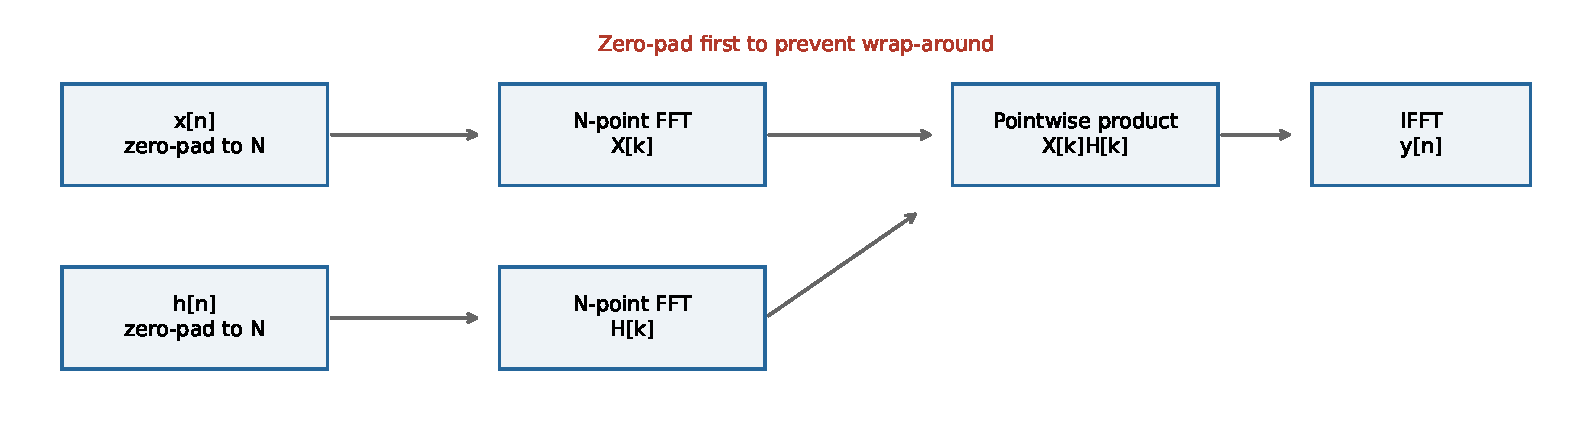
\includegraphics[width=0.96\textwidth]{07-dtft/fft-convolution-flow.pdf}
  \caption{用 FFT 计算线性卷积的流程。两个序列先补零到同一长度，再分别变换、逐点相乘，最后作逆变换。补零长度不足时，线性卷积的尾部会在循环卷积中折回。}
  \label{fig:fft-convolution-flow}
\end{figure}

\begin{pitfall}
  “频域相乘等于时域卷积”需要先看卷积的边界。DTFT 对应普通线性卷积；有限点 DFT 的逐点相乘对应 $N$ 点循环卷积。用 FFT 计算线性卷积时，\blue{补零长度必须满足}\cref{eq:fft-zero-padding}，否则得到的只是发生了折回的循环结果。
\end{pitfall}

\endgroup
